\documentclass[Master, ngerman, UKenglish]{scrbook}
%------------------------------------------------------------------------------
% This file contains a skeleton thesis for
% a Physics or Astronomy Institute in the University of Bonn

% Specify the thesis type as an option: PhD, Master, Diplom, Bachelor
% Specify the thesis stage as an option: Draft (default), Submit, Final, PILibrary

% Specify the language(s) in the class and then use babel.
% If you need more than one language, give the default language last,
% e.g. ngerman, UKenglish for a thesis in British (UK) English where you want
% to be able to set the language to German for some part of it.

%------------------------------------------------------------------------------
% Pass TeX Live version to the package
% Use command pdflatex --version to find out which version you are running
% Add option backref=false when your thesis is ready to turn off back-referencing
% in your bibliography
\usepackage[texlive=2016]{ubonn-thesis}
% Adjustments to standard biblatex style
\usepackage{ubonn-biblatex}

% Glossary package
% \usepackage[acronym,toc,nosuper]{glossaries}
% TikZ packages and libraries
% \usepackage{tikz}
% \usepackage{tikz-3dplot}
% \usepackage{pgfplots}
% \usetikzlibrary{positioning,shapes,arrows}
% \usetikzlibrary{decorations.pathmorphing}
% \usetikzlibrary{decorations.markings}
\usepackage{thesis_defs}

%------------------------------------------------------------------------------
% Instead of colouring  links, cites, table of contents etc.
% put them in a coloured box for the screen version.
% This is probably a good idea when you print your thesis.
% \hypersetup{colorlinks=false,
%   linkbordercolor=blue,citebordercolor=magenta,urlbordercolor=darkgreen
% }

%------------------------------------------------------------------------------
% When writing your thesis it is often helpful to have the date and
% time in the output file. Comment this out for the final version.
\ifoot[\today{} \thistime]{\today{} \thistime}

% In order to check if your labels are referenced try the refcheck package
% \usepackage{refcheck}

%------------------------------------------------------------------------------
% biblatex is included by ubonn-thesis. Look there for the settings used.
% See the options for settings that can be changed easily.
% For further changes copy the \RequirePackage[...]{biblatex} here
% and include ubonn-thesis with the option biblatex=false.

% Specify the bibliography files here and not at the end!
% Use standard_refs-bibtex if you use bibtex or bibtex8
% and standard_refs-biber  if you use biber
\addbibresource{bib/thesis_refs.bib}
\addbibresource{bib/standard_refs-biber.bib}

%------------------------------------------------------------------------------
% The following definitions are used to produce the title pages
% needed at various stages
\newcommand{\thesistitle}{Title of the Thesis}
\newcommand*{\thesisauthor}{Author's name}
\newcommand*{\thesistown}{Place of birth}
\renewcommand*{\InstituteName}{\PI}
\renewcommand*{\inInstitute}{\inPI}
\renewcommand*{\InstituteAddress}{\PIaddress}
% Adjust \thesisreferee...text depending on male/female referee
\newcommand*{\thesisrefereeonetext}{1.\ Gutachter}
\newcommand*{\thesisrefereeone}{Prof.\ Dr.\ John Smith}
\newcommand*{\thesisrefereetwotext}{2.\ Gutachterin}
\newcommand*{\thesisrefereetwo}{Prof.\ Dr.\ Anne Jones}
% Date when thesis was submitted (Master/Diplom)
% Year or Month, Year when thesis was submitted (PhD)
\newcommand*{\thesissubmit}{XX.YY.2018}
% \newcommand*{\thesissubmit}{Month 2018}
% Date of thesis examination (PhD)
\newcommand*{\thesispromotion}{XX.YY.2018}
% Month and year of the final printed version of the thesis
\newcommand*{\thesismonth}{MMM}
\newcommand*{\thesisyear}{2018}
\newcommand*{\thesisnumber}{BONN-IR-2018-XXX}

%------------------------------------------------------------------------------
% The abstract is only needed for the printed version and should be in
% English regardless of the language of the thesis
\newcommand{\thesisabstract}{%
  \begin{otherlanguage}{UKenglish}
    This is your thesis abstract. It may be in a language that is
    different from the rest of your thesis.
  \end{otherlanguage}
}

%------------------------------------------------------------------------------
% \includeonly can be used to select which chapters you want to process
% A simple \include command just inserts a \clearpage before and after the file
% Note that \includeonly can be quite picky! Do not forget to put a
% comma after the filename, otherwise it will simply be ignored!
% \includeonly{%
%   thesis_intro,
%   thesis_appendix,
%   thesis_acknowledge
% }

%------------------------------------------------------------------------------
% Give a list of directories where figures can be found. Do not leave
% any spaces in the list and end the directory name with a /
\graphicspath{%
  {figs/}%
  {figs/cover/}%
}

%------------------------------------------------------------------------------
% Make a glossary and a list of acronyms
% \makeglossaries

% Glossary entries
% \input{thesis_glossary}

% Draft version - add the word DRAFT on the cover pages
\ifthenelse{\equal{\ThesisVersion}{Draft}}{%
  \usepackage{background}
  \ifthenelse{\texlive < 2013}{%
    \SetBgContents{DRAFT}
    \SetBgColor{blue!30}
  }{%
    \backgroundsetup{contents=DRAFT, color=blue!30}
  }
}

%------------------------------------------------------------------------------
\begin{document}

% Cover page of thesis - this is only needed for the printed final
% version to be submitted to the department library
% Do not use this page for thesis submission to the Prüfungsamt or Promotionsbüro!
\ifthenelse{\equal{\ThesisVersion}{PILibrary}}{%
  \typeout{Document \jobname, Info: PI library version of thesis}
  \input{../cover/\ThesisType_Cover}
}{}

% Start counting pages from the title page
\frontmatter
% Dedication has to come before \maketitle
% \dedication{Dedicated to no one}

% Select the correct title page(s)
\ifthenelse{\equal{\ThesisType}{Unknown}}{%
  \typeout{Document \jobname, Error: Unknown thesis type - no title page printed}
}{%
  % Bachelor thesis only has one title page
  \ifthenelse{\equal{\ThesisType}{Bachelor}}{%
    \typeout{Document \jobname, Info: Bachelor thesis}
    \input{../cover/\ThesisType_Title}
  }{%
    \ifthenelse{\equal{\ThesisVersion}{Final} \OR \equal{\ThesisVersion}{PILibrary}}{%
      % Final and PI library versions
      \typeout{Document \jobname, Info: Final version of a \ThesisType  thesis}
      \input{../cover/\ThesisType_Final_Title}
    }{% Submission and draft versions
      \input{../cover/\ThesisType_Submit_Title}
      \typeout{Document \jobname, Info: Draft/submission version of a \ThesisType  thesis}
    }
  }
}

\pagestyle{scrplain}

%------------------------------------------------------------------------------
% You can add your acknowledgements here - don't forget to also add
% them to \includeonly above
%------------------------------------------------------------------------------
\chapter{Acknowledgements}
\label{sec:acknowledgements}
%------------------------------------------------------------------------------
In 2017, I had the fortune to come to Germany and study physics. This would not have been possible without Bonn-Cologne Graduate School, so I would like to thank the admission committee for giving me an opportunity to pursue my master degree in physics.

I would like to thank Prof.\ Dr.\ Ian C.\ Brock for giving me an opportunity to write my thesis in his group. There is no doubt that without his guidance, wisdom and direction over the course of my degree, this thesis would not have been possible. I would also like to thank Prof.\ Dr.\ Florian Bernlochner, who agreed to be my second referee for this thesis.

Furthermore, I would like to thank Prof.\ Dr.\ Heiko Lacker, Dr.\ Janet Dietrich and Ferdinand Schenck from the Berlin VLQ group for helping me to understand the analysis better and also for their fruitful discussions on my results.

A big thanks to Anjishnu Bandyopadhyay for his support right from the beginning, when he introduced me VLQs till the last day of my submission. I truly appreciate all of his efforts for helping me with all my queries irrespective of the time on the clock as well as the priceless discussions on physics-related topics during DPG and at CERN. It has been a pleasure working with him. I would also like to thank Dr.\ Regina Moles Valls and Dr.\ Rui Zhang for their guidance and motivation when I initially joined this group as an intern. I would like to thank Dr.\ Oleh Kivernyk for his valuable suggestions on my results on the ABCD method.

Next, I would like to thank Federico G.\ D.\ Capriles for proofreading my first draft of this thesis and giving me some good memories of card game evenings. I would also like to thank Tanja Holm for the priceless discussions on jets and Christian Kirfel for the general discussions on machine learning related topics as well as teaching me some basic German culture. I would also like to thank Chris Boever for always motivating me and constantly reminding me that I am the next one after him. I am also grateful to him for proofreading some parts of my first draft of this thesis. I would like to thank Hanna We for all the interesting discussions we had on Indian and Korean cultures while sharing the same office. A special thanks to all the other members of the Brock group who were in the group during my days there, including but not limited to Nilima, Nicolas, Piet, Ellinor, Richard.

I would also like to thank everyone in the Desch group for the discussions during the Jamborees. A special thanks to all my friends and colleagues without them, my experience during my degree would not be as enjoyable.

Finally, I would like to thank my parents and family who are \SI{6000}{\kilo\meter} away from me but still their unconditional love and unlimited support encouraged me to start my venture; without them, it would not have been possible for me to manage and finish my studies.


%%% Local Variables: 
%%% mode: latex
%%% TeX-master: "../mythesis"
%%% End: 


\tableofcontents

\mainmatter
\pagestyle{scrheadings}

% Turn off DRAFT for the following pages
\ifthenelse{\equal{\ThesisVersion}{Draft}}{%
  \ifthenelse{\texlive < 2013}{%
    \SetBgContents{}
  }{%
    \backgroundsetup{contents={}}
  }
}{}

%------------------------------------------------------------------------------
% Add your chapters here - don't forget to also add them to \includeonly above
% !TEX root = mythesis.tex

%==============================================================================
\chapter{Introduction}
\label{sec:intro}
%==============================================================================
\textit{“Not only is the Universe stranger than we think, it is stranger than we can think.”} - Werner Heisenberg

\vspace{0.5cm}
The formation of the universe is explained by cosmological and particle physics models. The field of high energy physics tries to understand the nature and the formation of the universe. It was started in 1897 when the discovery of electron~\cite{electron} let humanity to step into the subatomic scale. Later on, the quantum mechanics and general relativity were established well enough to answer the open questions which pushed the boundaries of the scientific limits further. The two theories which can precisely describe the universe are the Standard Model on particle physics (SM) and the Lambda Cold Dark Matter ($\Lambda$CDM) model of cosmology. These theories are confirmed to high precision by the Large Hadron Collider (LHC) and the Planck Mission~\cite{planck} experiments. The LHC was built from 1998 to 2008~\cite{lhc} to collide high-energy protons to probe the behaviour of the particles.

A great milestone in the history of particle physics was reached when the Higgs boson was discovered by the ATLAS~\cite{higgsatlas} and CMS~\cite{higgscms} experiments at the LHC in 2012. It was the last piece of the Standard Model to be discovered. With this, the Standard model is considered to be the most fundamental theory, which is accurate and precise in all of its predictions. However, the fact is that it is still not a complete theory because of the limitation of not able to explain some important phenomena. One of them is the instability of the mass of the Higgs boson. The radiative corrections to the mass of the Higgs boson conflict with the experimental value of the Higgs boson mass, which is $\SI{125.7}{\giga\electronvolt}$~\cite{higgsatlas}~\cite{higgscms}. These corrections quadratically diverge up to the cut-off scale of new physics. This is known as the Higgs mass hierarchy problem. This leads physicists to think beyond the scope of the Standard Model. There are various theories which are proposed to explain this phenomenon. Some of these theories predict the existence of an exotic particle called vector-like quark (VLQ) which couples with the Standard Model third generation quarks. VLQ can solve the Higgs mass hierarchy problem by introducing an additional loop correction which cancels out the divergence of these corrections. The search for VLQ is carried out in both ATLAS and CMS data collected so far from $pp$ collisions at the LHC. VLQ can either be produced singly or in pair. The single VLQ production is a dominant process at high VLQ masses~\cite{wulzer}. In this thesis, the single production of two such types of VLQs, $T$ and $Y$ quark are presented in $T/Y\rightarrow Wb$ analysis.

The main topic discussed in this thesis is the background estimation in the all-hadronic channel of $T/Y\rightarrow Wb$ analysis by using a data-driven method. This thesis is organised as follows. A brief introduction of the theoretical concepts which are important in particle physics is given in Chapter \ref{sec:theory}. A description of the Standard Model is provided and familiarises the reader with the idea of vector-like quarks. In Chapter \ref{sec:lhcandatlas}, an overview of the LHC accelerator and a detailed description of the ATLAS detector are given. Jets and its reconstruction algorithm are discussed in Chapter \ref{sec:jetsandtaggers}. The two different types of jet algorithms are also discussed in detail which are used in this thesis. In Chapter \ref{sec:analysisstrategy}, the strategy used for this analysis is described, including the study of all the possible backgrounds, data preparation for the analysis and the selection of interesting events. The topics essential to physics analyses, such as a description of the data and Monte Carlo samples used and reconstruction of physics objects with the ATLAS detector are also covered. An introduction to a data-driven method called the ABCD method is given in Chapter \ref{sec:abcd}. The ABCD method is used to estimate the multijet background.  An overview of the method and its implementation on the data along with the further approaches to improve the estimate are shown in this chapter. In Chapter \ref{sec:uncertainty_result}, all the uncertainties which are taken into account while performing the multijet estimation are described, which include both statistical and systematic uncertainties. In Chapter \ref{sec:results}, the final result of the multijet estimate, including all the uncertainties is presented. A comparison between the performances of different $W$-taggers and the jet collections are also shown. Finally, in Chapter \ref{sec:conclusion}, a brief summary and the concluding remarks about the research that is documented in this thesis are provided.


%%% Local Variables: 
%%% mode: latex
%%% TeX-master: "mythesis"
%%% End: 

% Uncomment the following command to get references per chapter.
% Put it inside the file or change \include to \input if you do not want the references
% on a separate page
% \printbibliography[heading=subbibliography]

%------------------------------------------------------------------------------
% Use biblatex for the bibliography
% Add bibliography to Table of Contents
% Comment out this command if your references are printed for each chapter.
\printbibliography[heading=bibintoc]

%------------------------------------------------------------------------------
% Include the following lines and comment out \printbibliography if
% you use BiBTeX for the bibliography.
% If you use biblatex package the files should be specified in the preamble.
% \KOMAoptions{toc=bibliography}
% {\raggedright
%   \bibliographystyle{../refs/atlasBibStyleWithTitle.bst}
%   % \bibliographystyle{unsrt}
%   \bibliography{./thesis_refs,../refs/standard_refs-bibtex}
% }

%------------------------------------------------------------------------------
\appendix
% \part*{Appendix}
% Add your appendices here - don't forget to also add them to \includeonly above
%------------------------------------------------------------------------------
\chapter{Control region distributions}
\label{sec:app}
%------------------------------------------------------------------------------
In this appendix, the distributions for all the kinematic and reconstructed variables from all the four control regions B, C, D and D1 are provided. 

In the control region, the other backgrounds are from the MC simulation and the multijet background is calculated from the equation below:

\begin{equation}
	N_{\text{j}}^{\text{Multijet}}[i] = N_{\text{j}}^{\text{Data}}[i] - N_{\text{j}}^{\text{Other bkg.}}[i] \,,
	\label{eqn:app}
\end{equation}
where $\text{j}\in\{\text{B, C, D, D1}\}$ and $i=$ bin.

Fig.\ \ref{fig:app:cr_b} shows all the six distributions from CR B. Fig.\ \ref{fig:app:cr_c} shows all the six distributions from CR C. Fig.\ \ref{fig:app:cr_d} shows all the six distributions from CR D. Fig.\ \ref{fig:app:cr_d1} shows all the six distributions from CR D1.

\begin{figure}[hbt!]
	\centering
	\graphicspath{{figs/appendix/CRB/}}
	\begin{subfigure}{.35\textwidth}
		\centering
		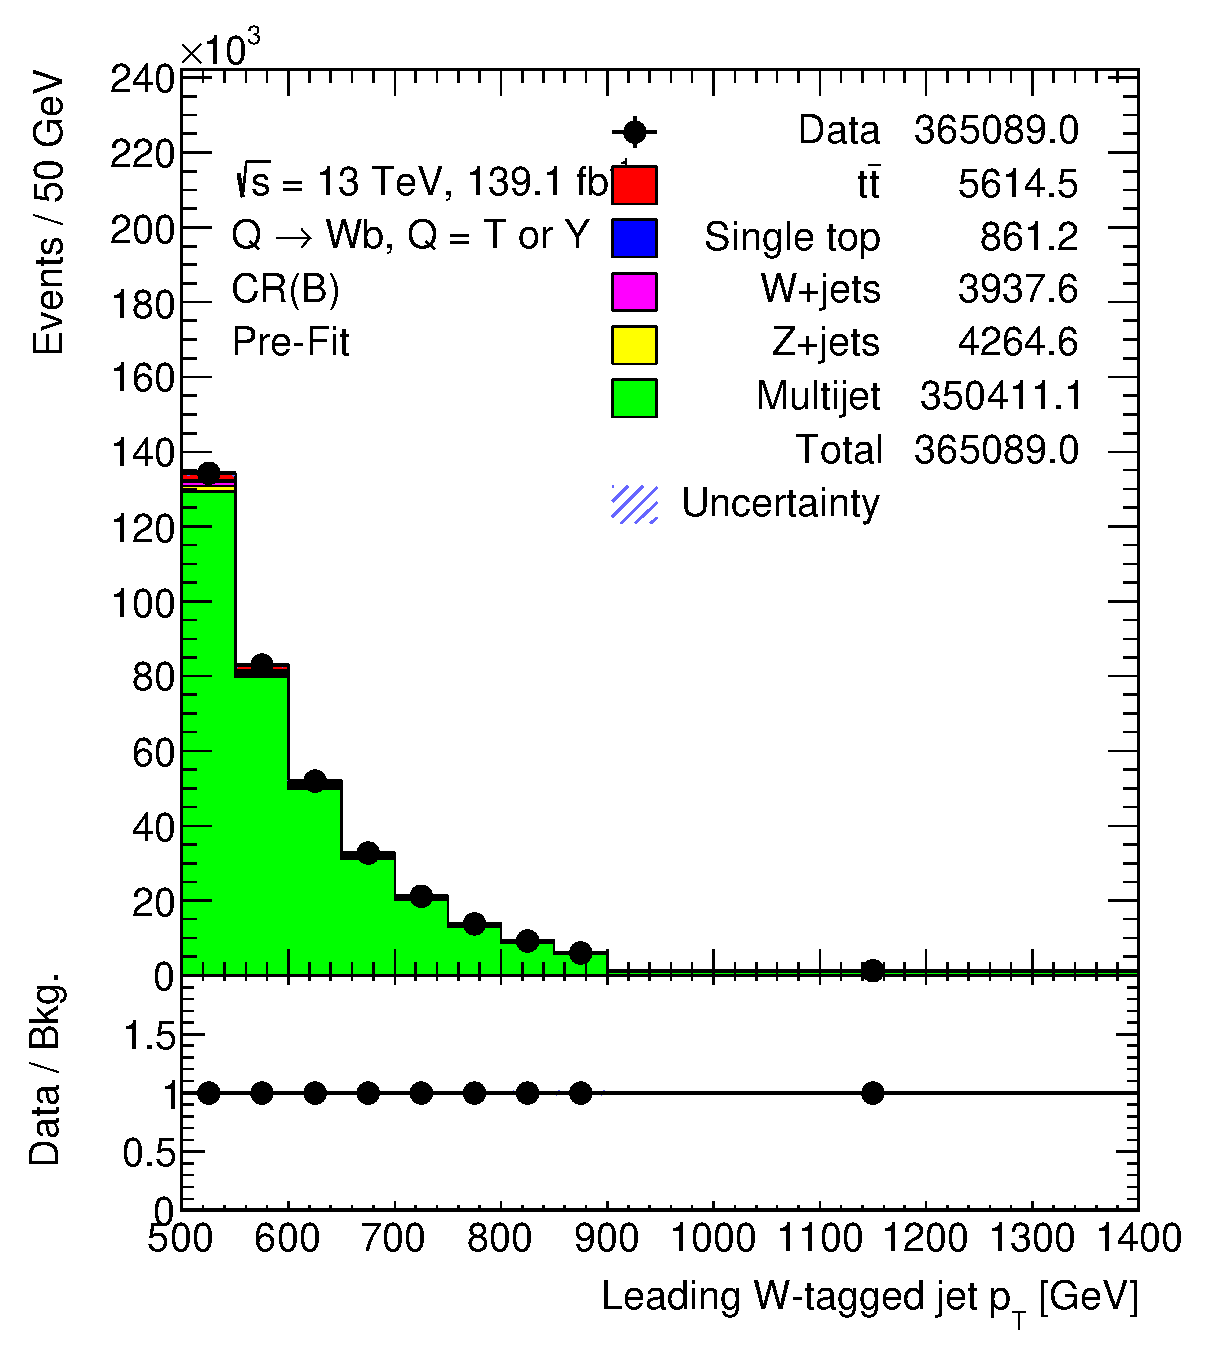
\includegraphics[width=\linewidth,height=\textheight,keepaspectratio]{CR_B_ljet_pt.eps}
		\caption{}
		\label{fig:app:cr_b:ljet_pt}
	\end{subfigure}\hspace{0.6cm}
	\begin{subfigure}{.35\textwidth}
		\centering
		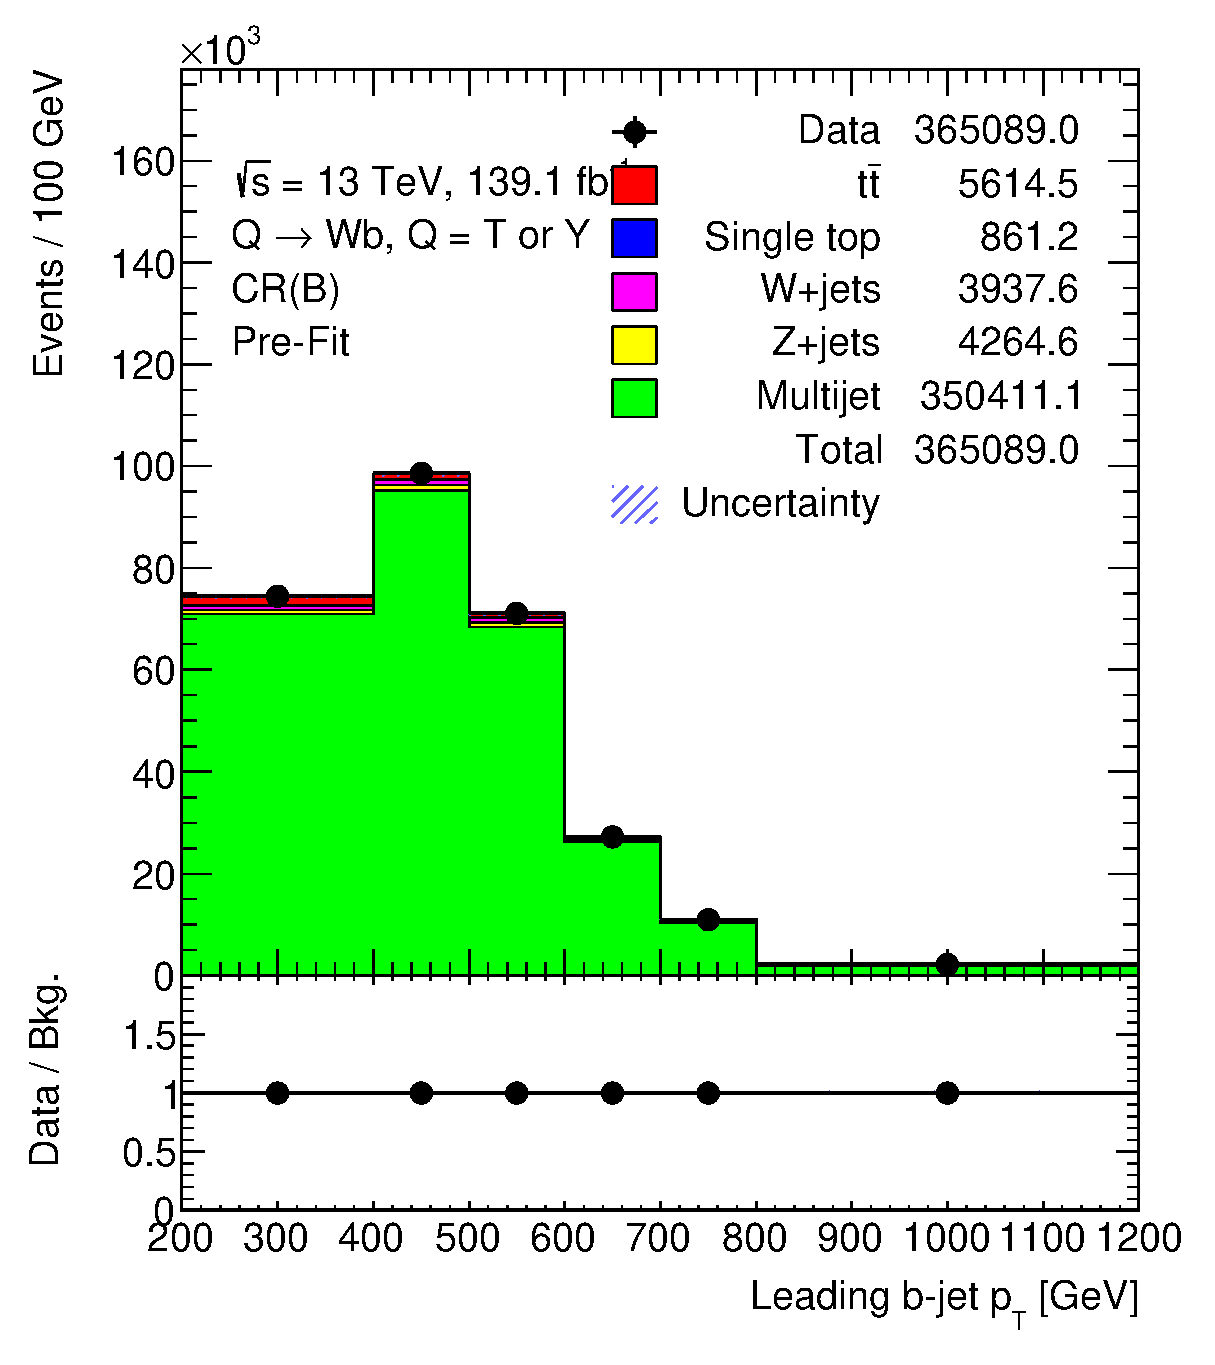
\includegraphics[width=\linewidth,height=\textheight,keepaspectratio]{CR_B_jet_pt.eps}
		\caption{}
		\label{fig:app:cr_b:jet_pt}
	\end{subfigure}
	\begin{subfigure}{.35\textwidth}
		\centering
		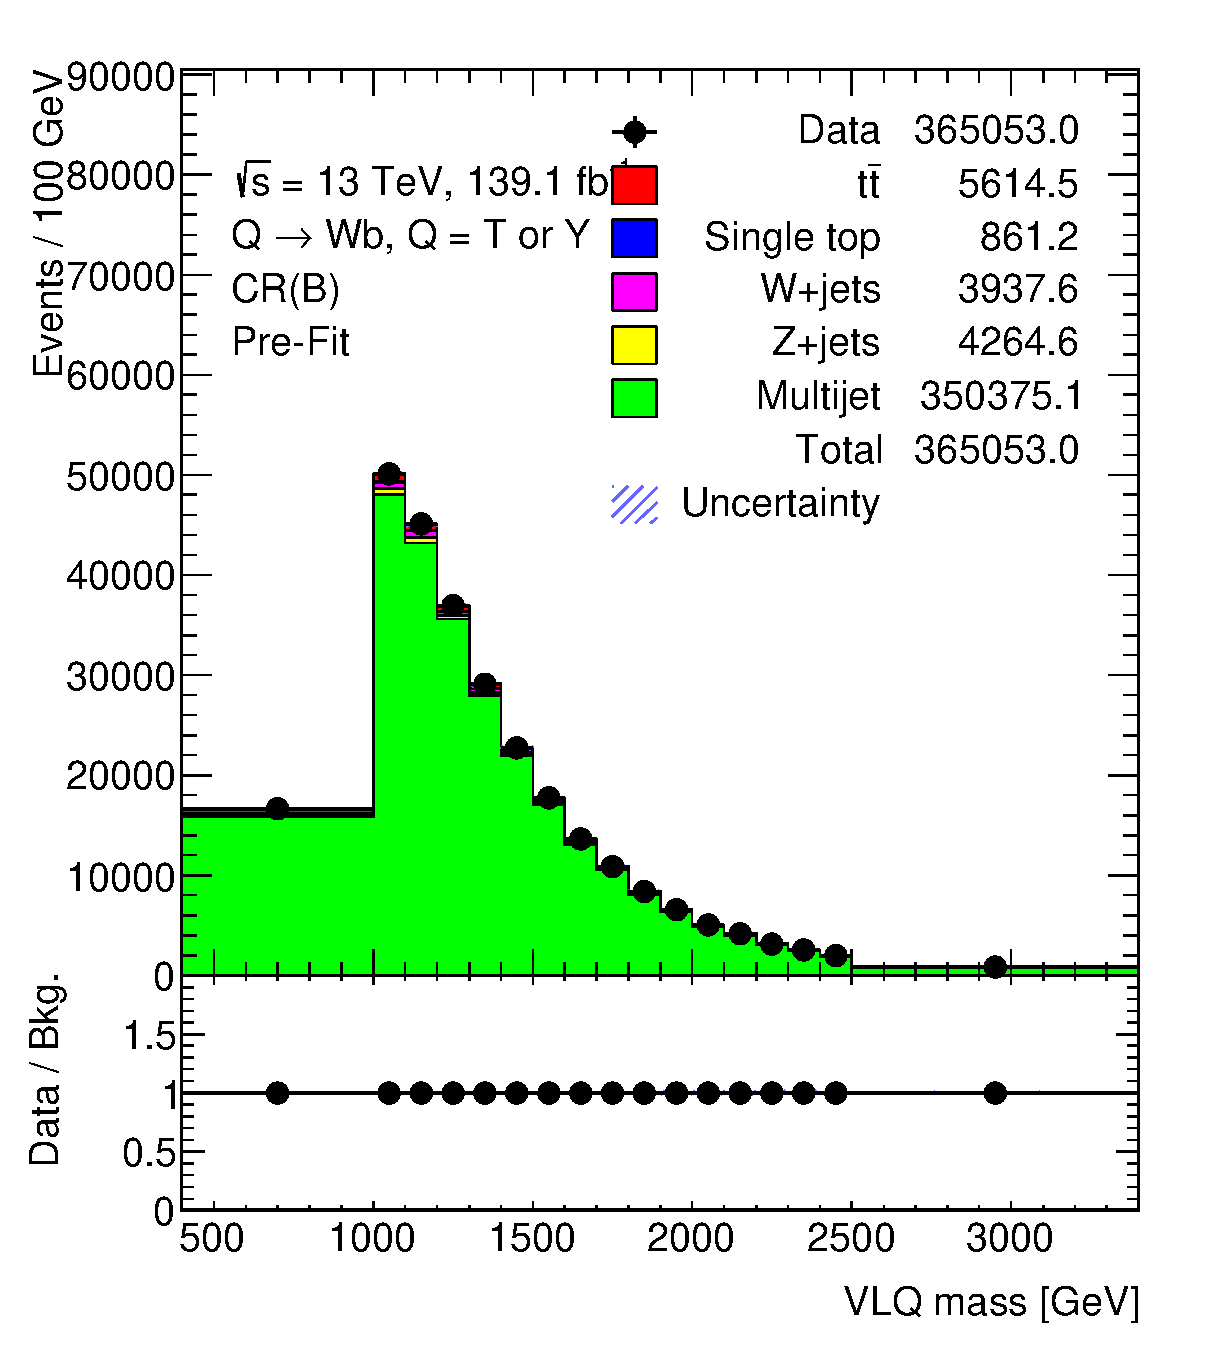
\includegraphics[width=\linewidth,height=\textheight,keepaspectratio]{CR_B_VLQM.eps}
		\caption{}
		\label{fig:app:cr_b:VLQM}
	\end{subfigure}\hspace{0.6cm}
	\begin{subfigure}{.35\textwidth}
		\centering
		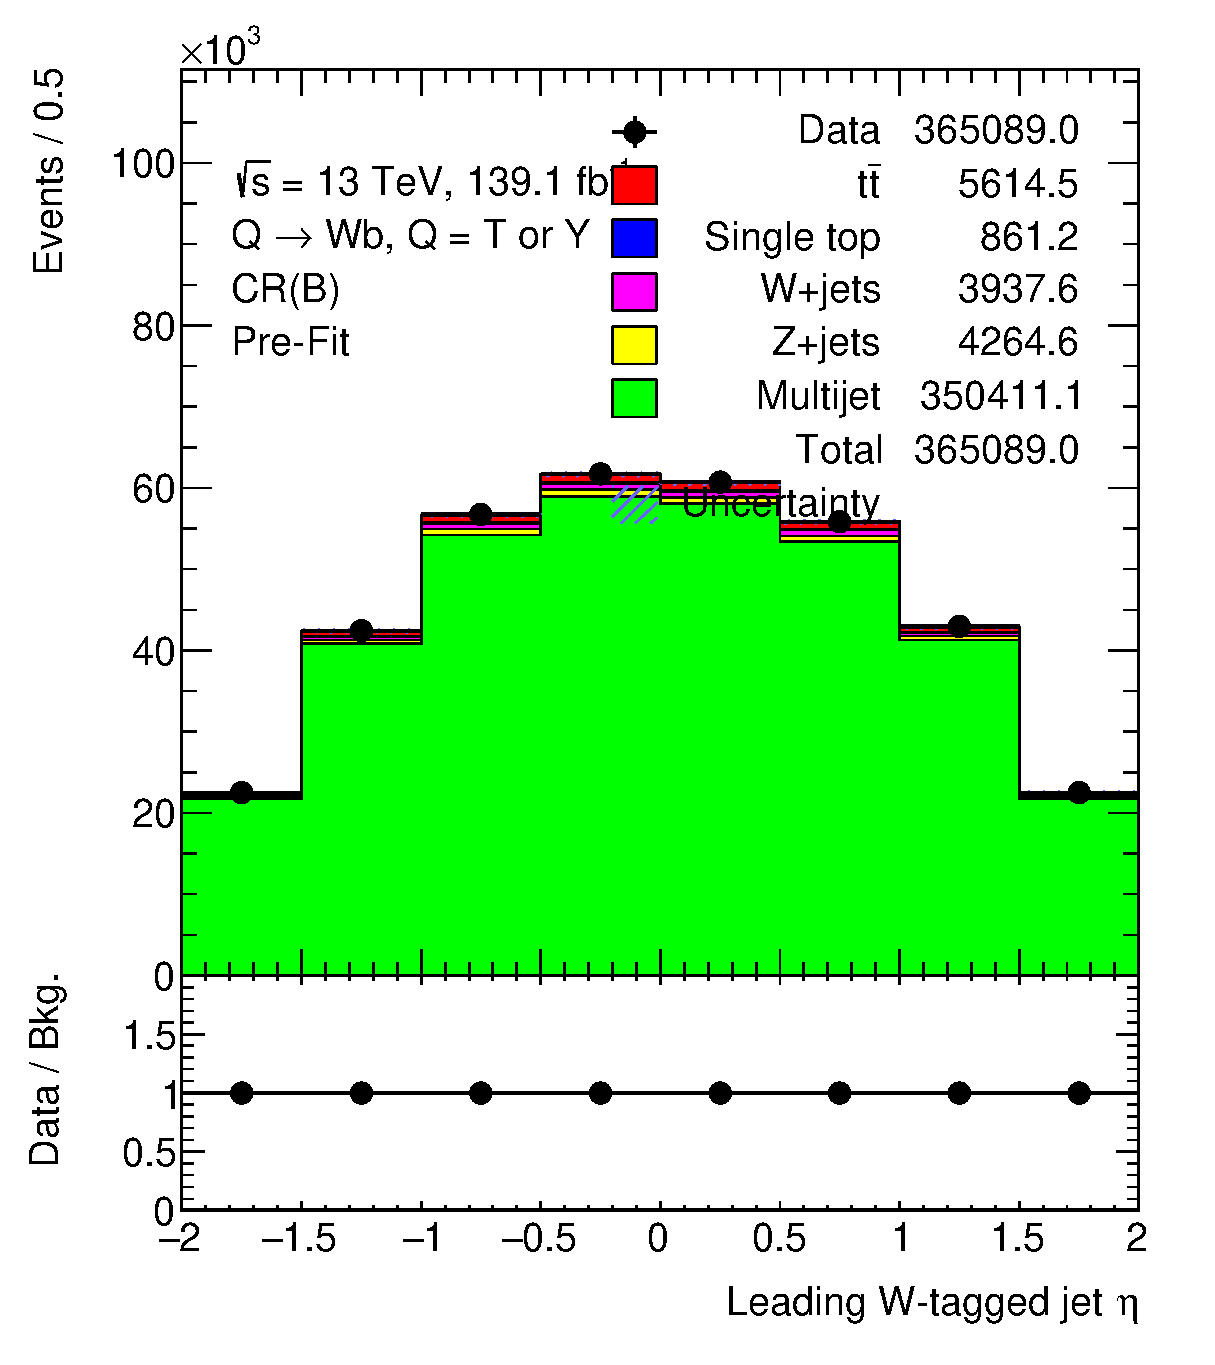
\includegraphics[width=\linewidth,height=\textheight,keepaspectratio]{CR_B_ljet_eta.eps}
		\caption{}
		\label{fig:app:cr_b:ljet_eta}
	\end{subfigure}
	\begin{subfigure}{.35\textwidth}
		\centering
		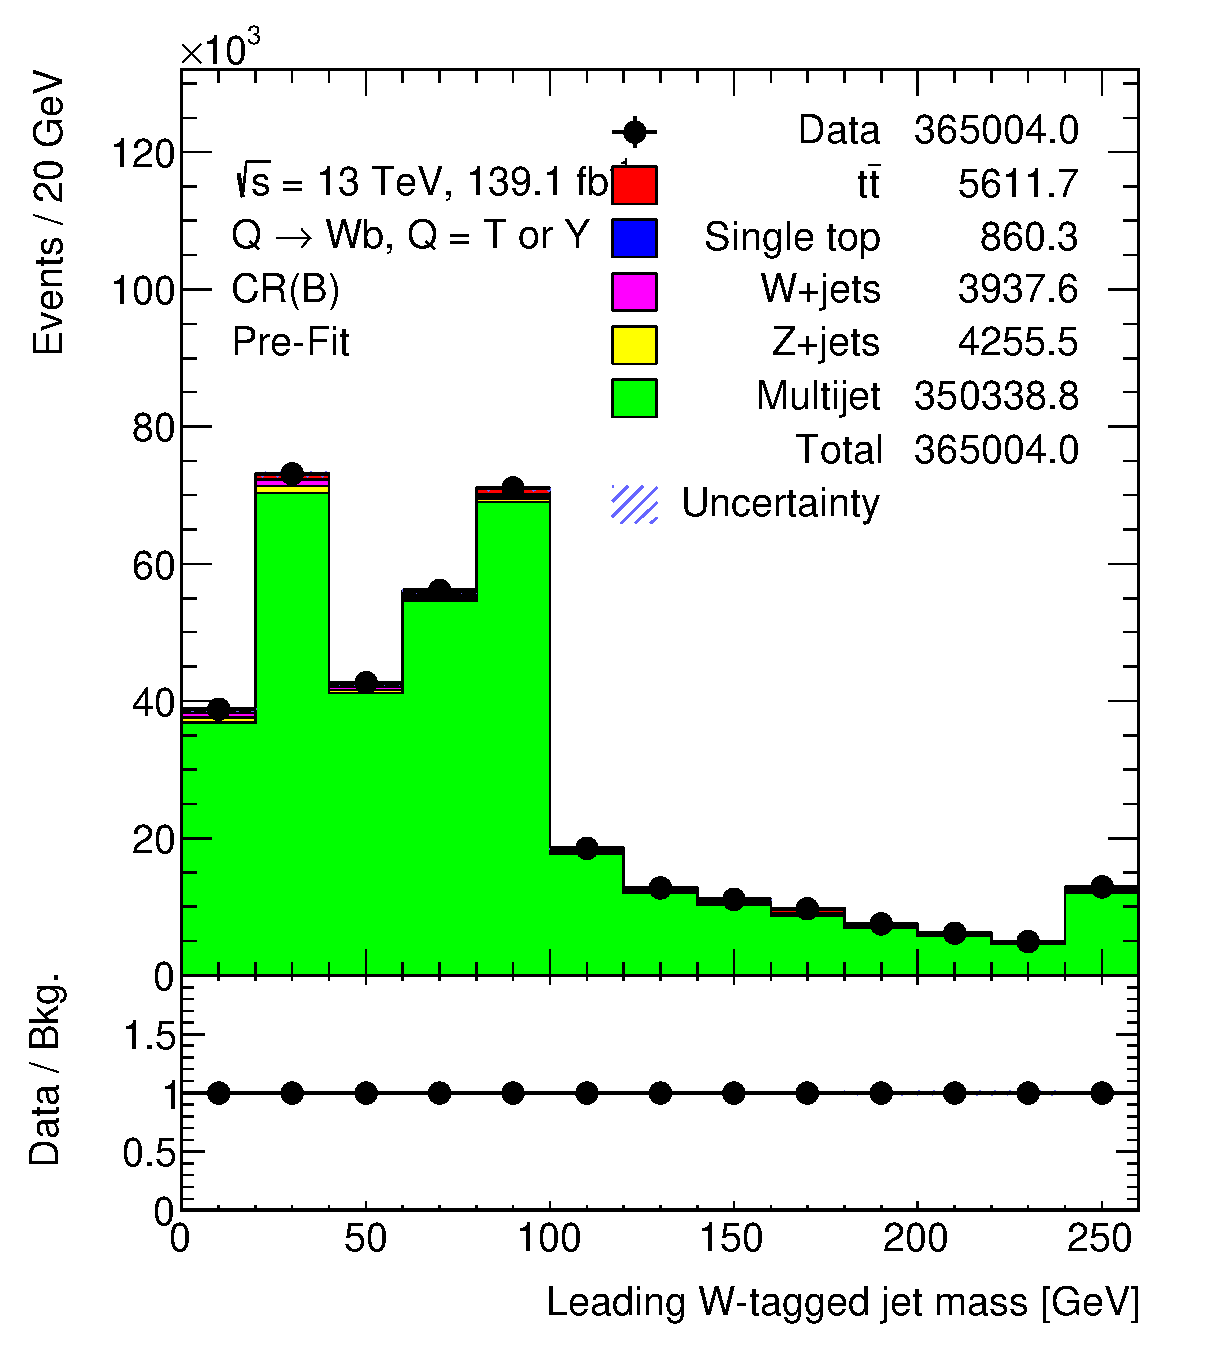
\includegraphics[width=\linewidth,height=\textheight,keepaspectratio]{CR_B_ljet_m.eps}
		\caption{}
		\label{fig:app:cr_b:ljet_m}
	\end{subfigure}\hspace{0.6cm}
	\begin{subfigure}{.35\textwidth}
		\centering
		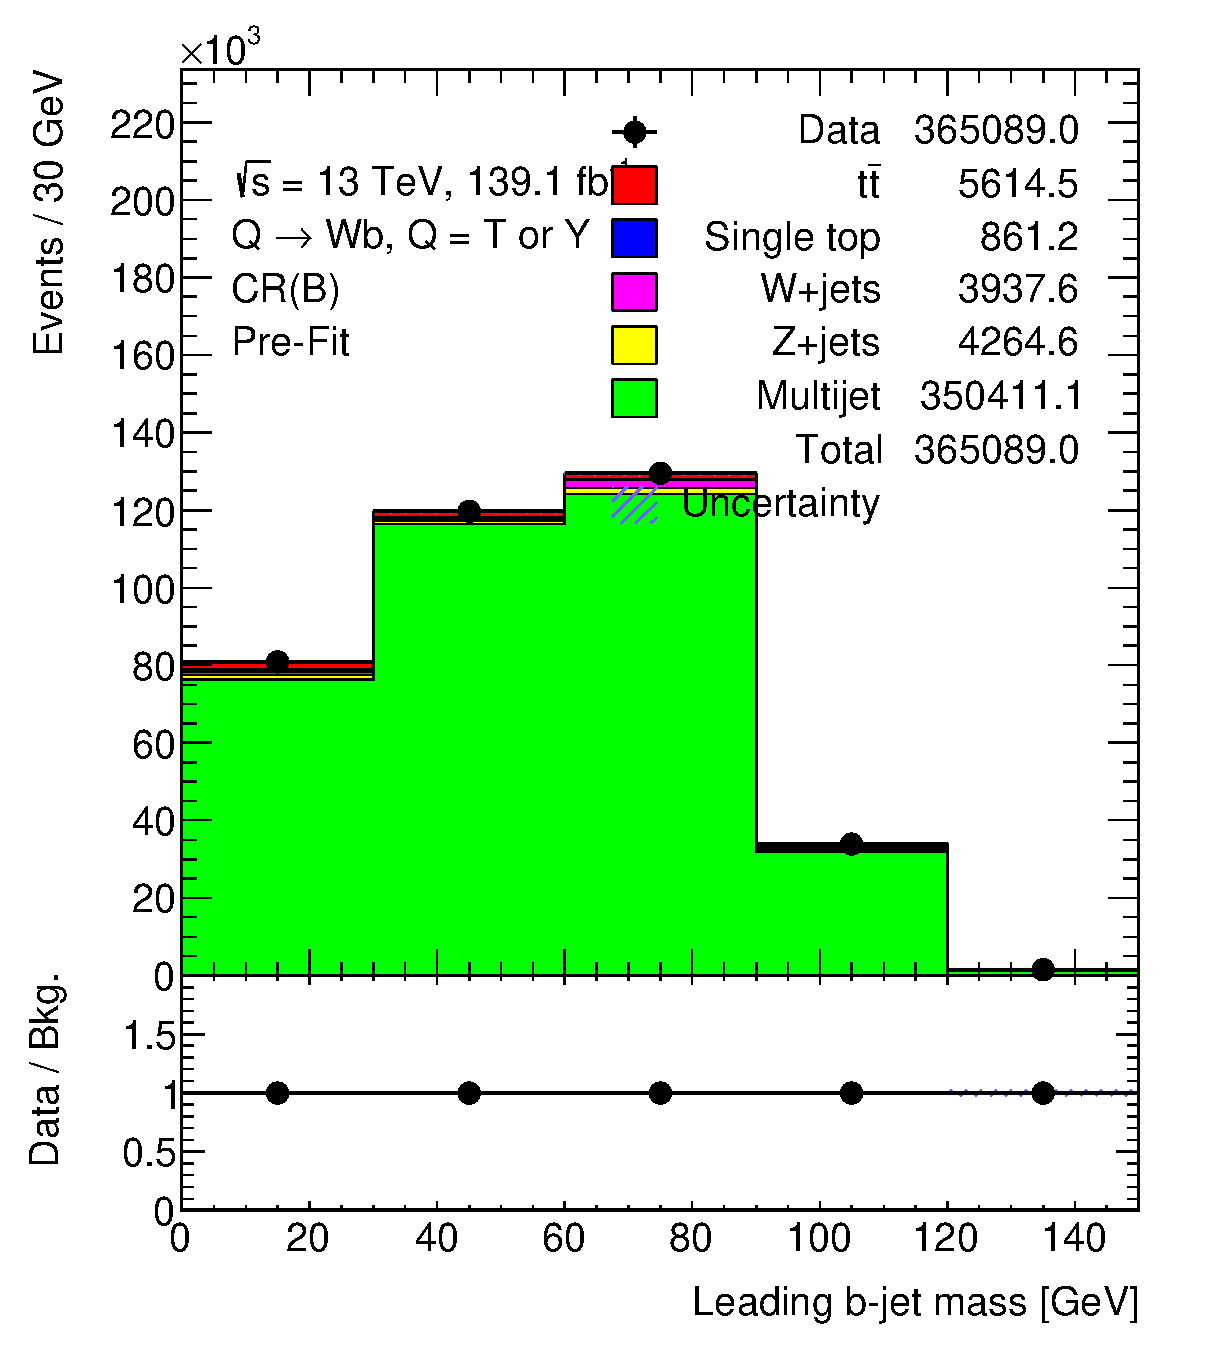
\includegraphics[width=\linewidth,height=\textheight,keepaspectratio]{CR_B_jet_m.eps}
		\caption{}
		\label{fig:app:cr_b:jet_m}
	\end{subfigure}
	\caption{A data/bkg.\ comparison of kinematic and reconstructed variables in CR B where the multijet background (in green) is calculated by Eqn.\ \ref{eqn:app} and the other backgrounds are from the MC simulation. The variables include (a) $p_{\text{T}}$ of $W$-tagged large-$R$ jet, (b) $p_{\text{T}}$ of leading $b$-tagged small-$R$ jet, (c) VLQ mass reconstructed from the kinematics of $W$-tagged large-$R$ jet and leading $b$-tagged small-$R$ jet, (d) $\eta$ distribution of $W$-tagged large-$R$ jet, (e) mass of $W$-tagged large-$R$ jet, and (f) mass of leading $b$-tagged small-$R$ jet.}
	\label{fig:app:cr_b}
\end{figure}







\begin{figure}[hbt!]
	\centering
	\graphicspath{{figs/appendix/CRC/}}
	\begin{subfigure}{.35\textwidth}
		\centering
		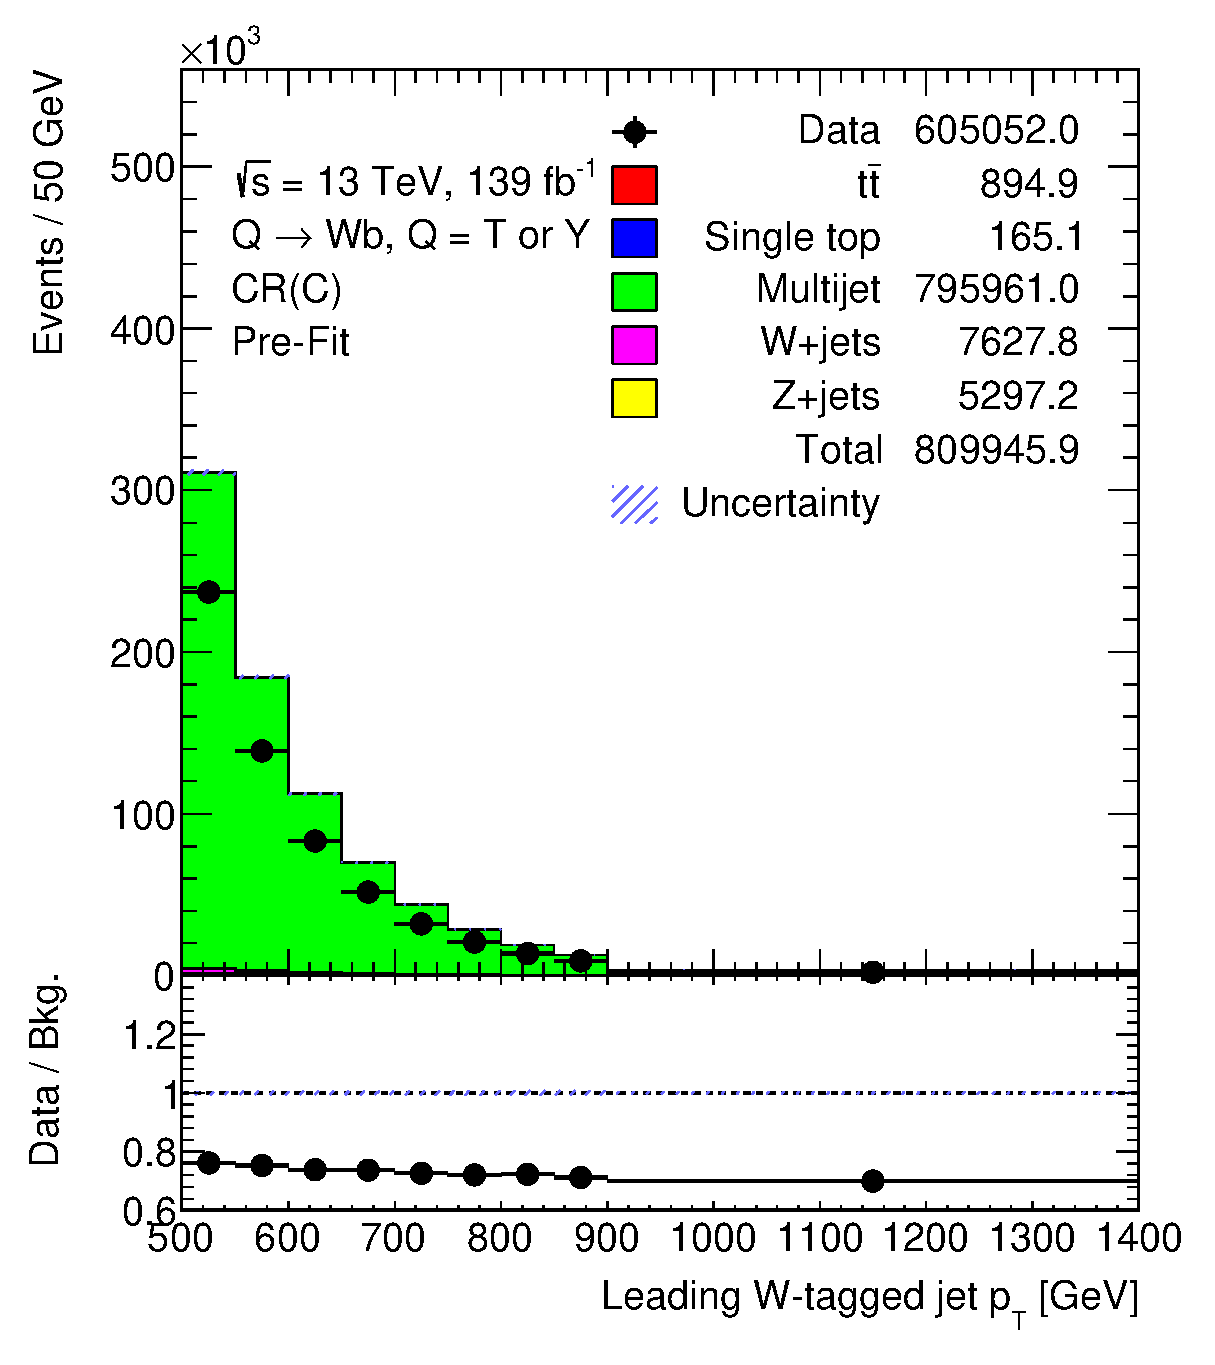
\includegraphics[width=\linewidth,height=\textheight,keepaspectratio]{CR_C_ljet_pt.eps}
		\caption{}
		\label{fig:app:cr_c:ljet_pt}
	\end{subfigure}\hspace{0.6cm}
	\begin{subfigure}{.35\textwidth}
		\centering
		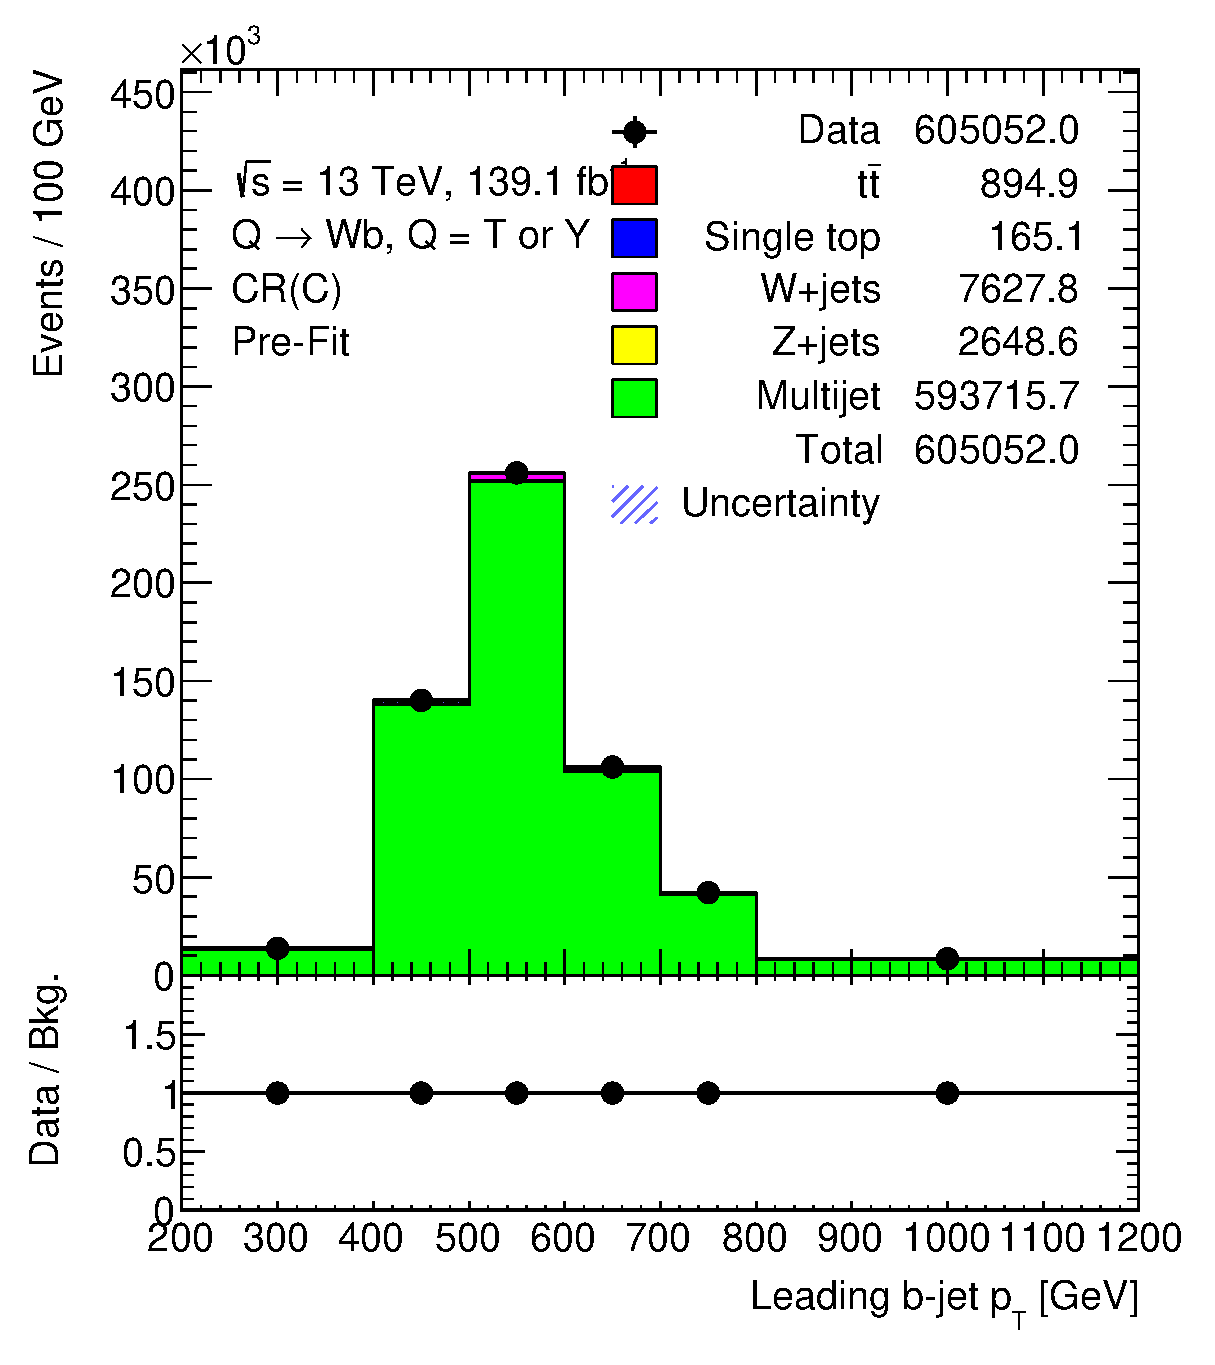
\includegraphics[width=\linewidth,height=\textheight,keepaspectratio]{CR_C_jet_pt.eps}
		\caption{}
		\label{fig:app:cr_c:jet_pt}
	\end{subfigure}
	\begin{subfigure}{.35\textwidth}
		\centering
		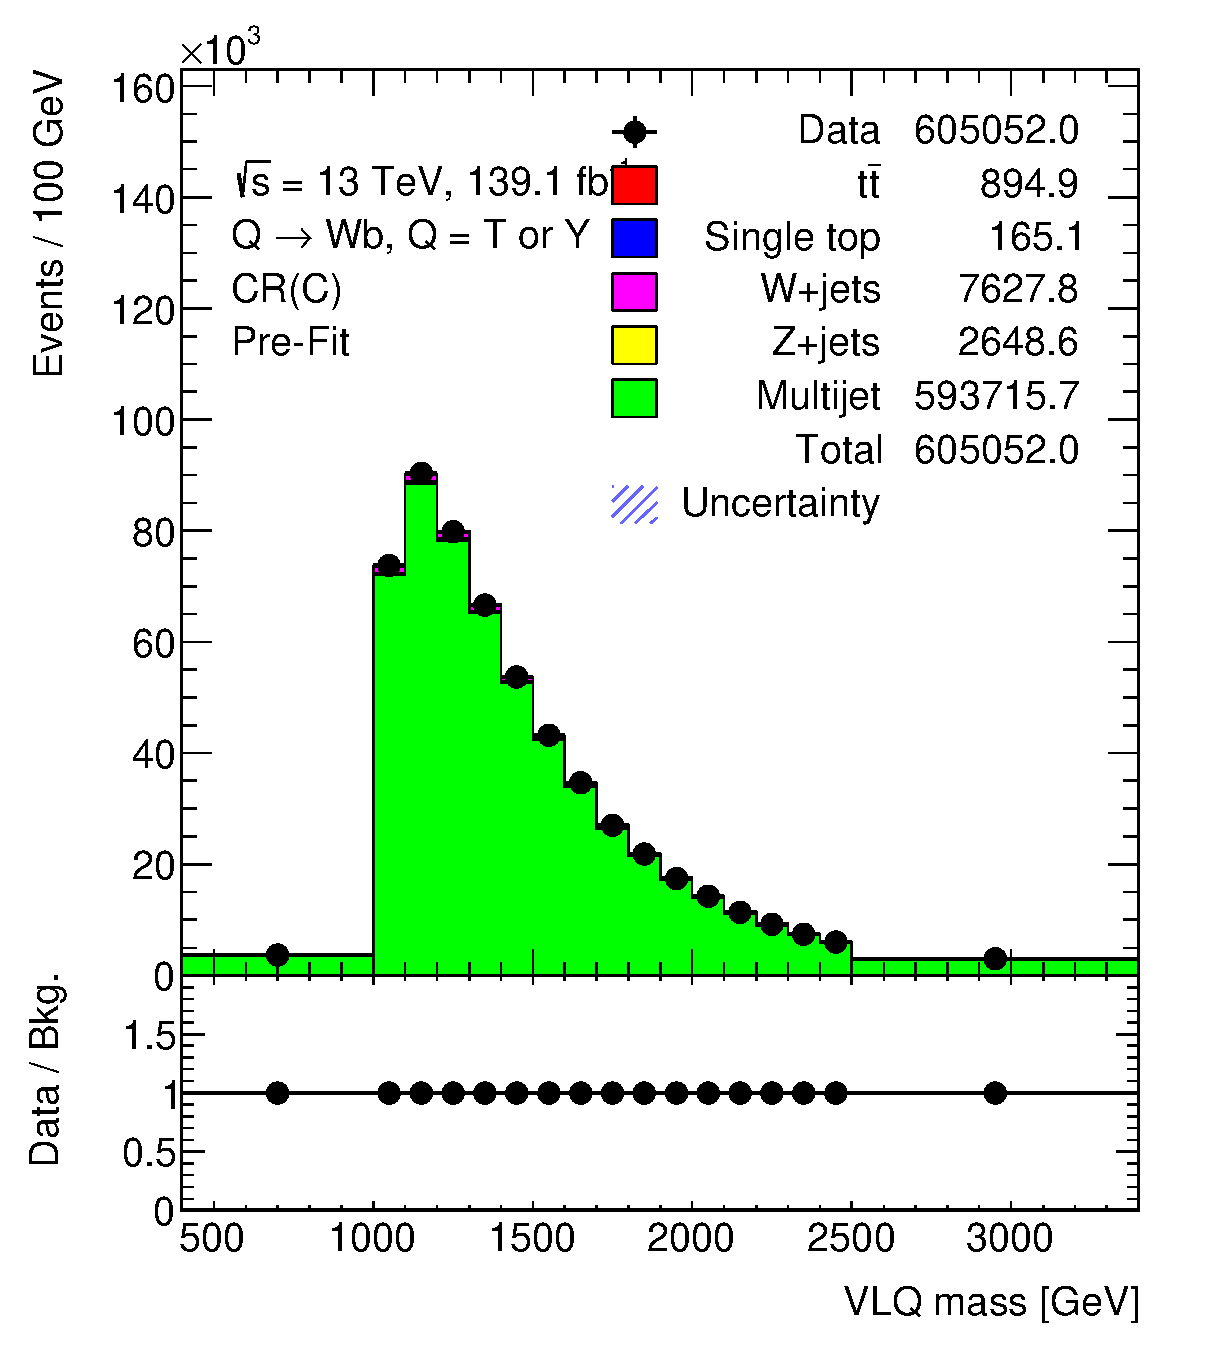
\includegraphics[width=\linewidth,height=\textheight,keepaspectratio]{CR_C_VLQM.eps}
		\caption{}
		\label{fig:app:cr_c:VLQM}
	\end{subfigure}\hspace{0.6cm}
	\begin{subfigure}{.35\textwidth}
		\centering
		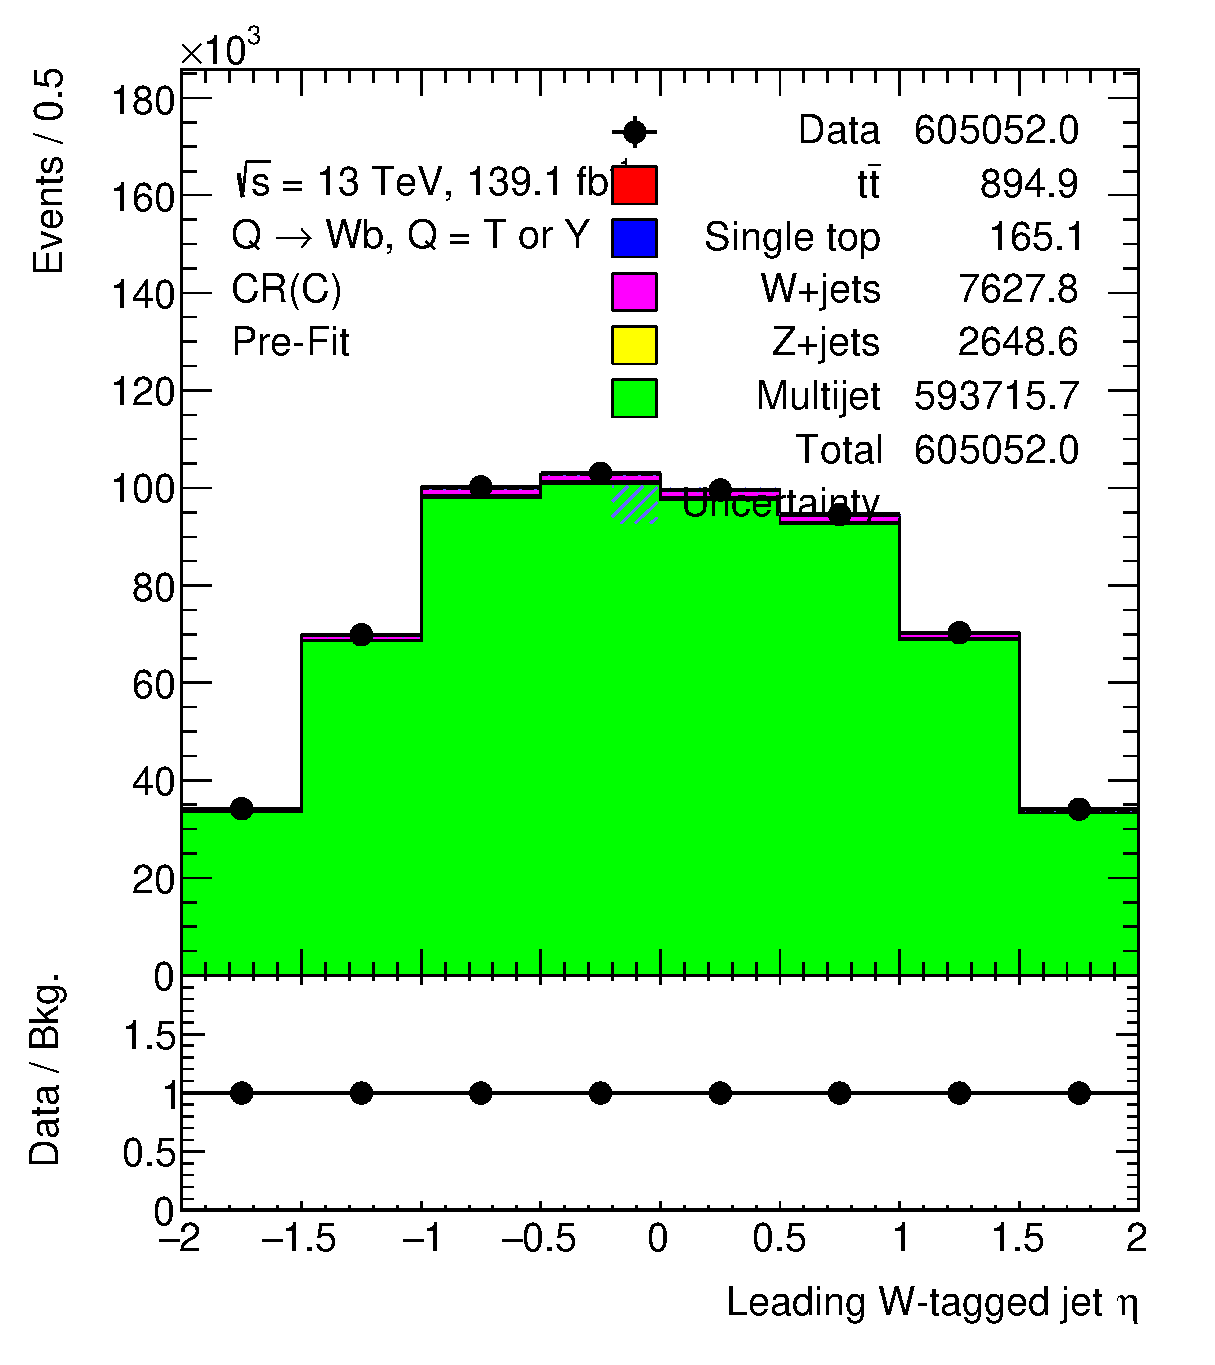
\includegraphics[width=\linewidth,height=\textheight,keepaspectratio]{CR_C_ljet_eta.eps}
		\caption{}
		\label{fig:app:cr_c:ljet_eta}
	\end{subfigure}
	\begin{subfigure}{.35\textwidth}
		\centering
		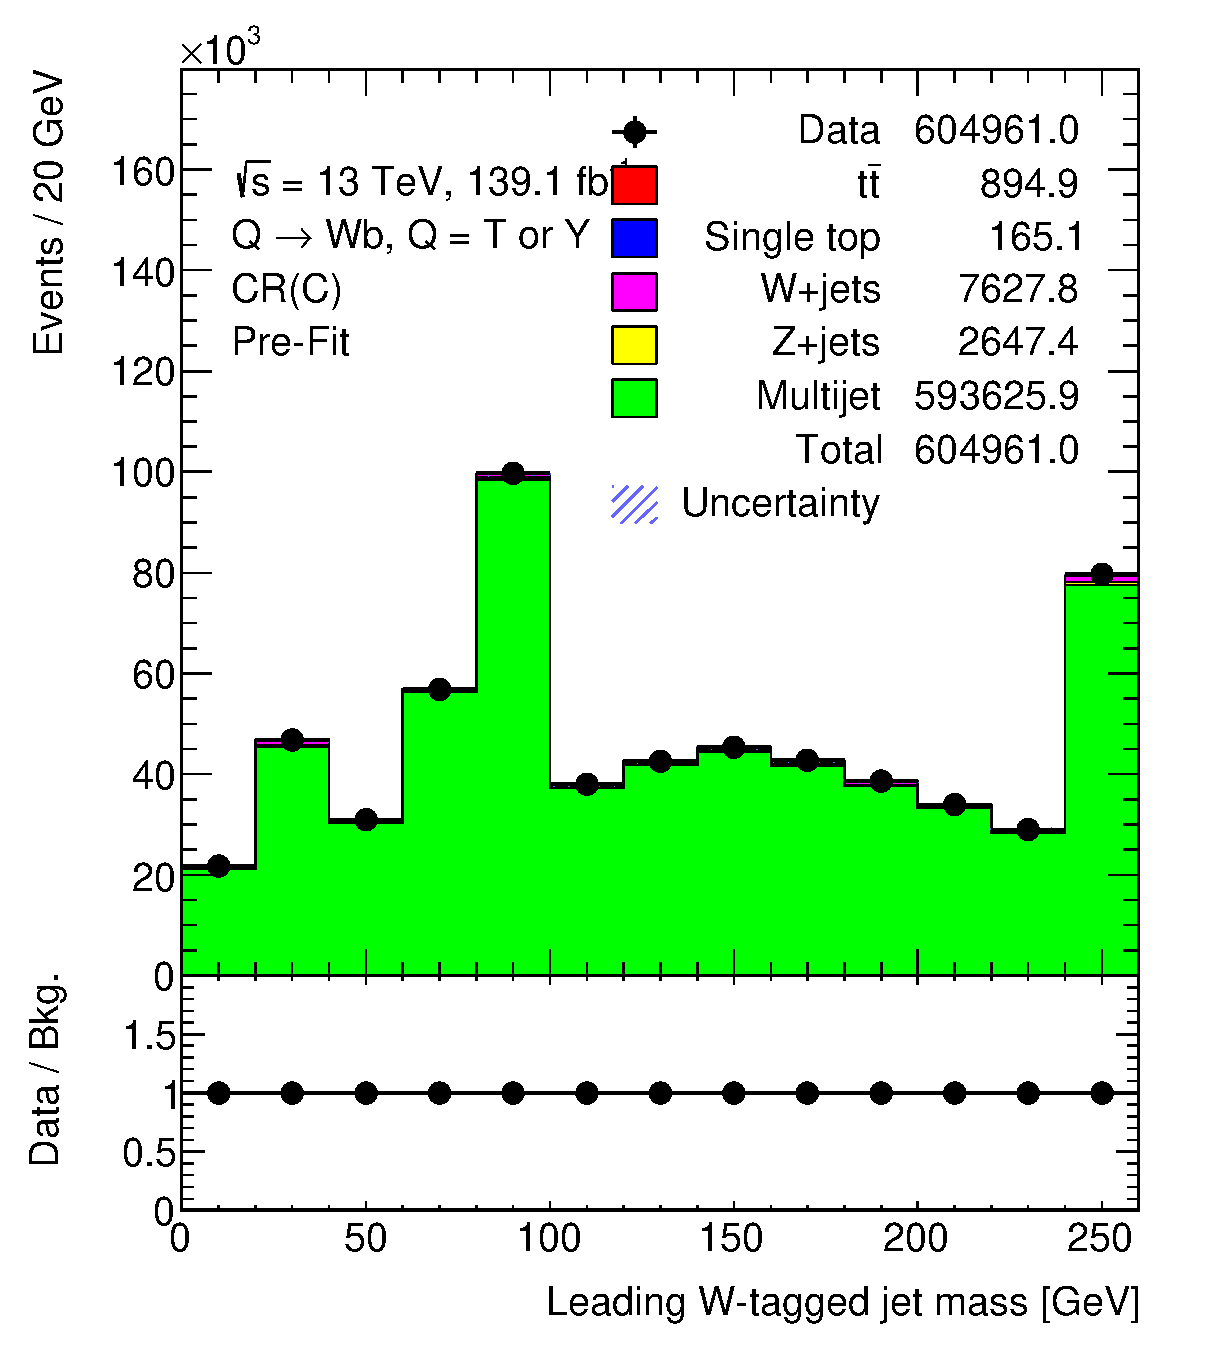
\includegraphics[width=\linewidth,height=\textheight,keepaspectratio]{CR_C_ljet_m.eps}
		\caption{}
		\label{fig:app:cr_c:ljet_m}
	\end{subfigure}\hspace{0.6cm}
	\begin{subfigure}{.35\textwidth}
		\centering
		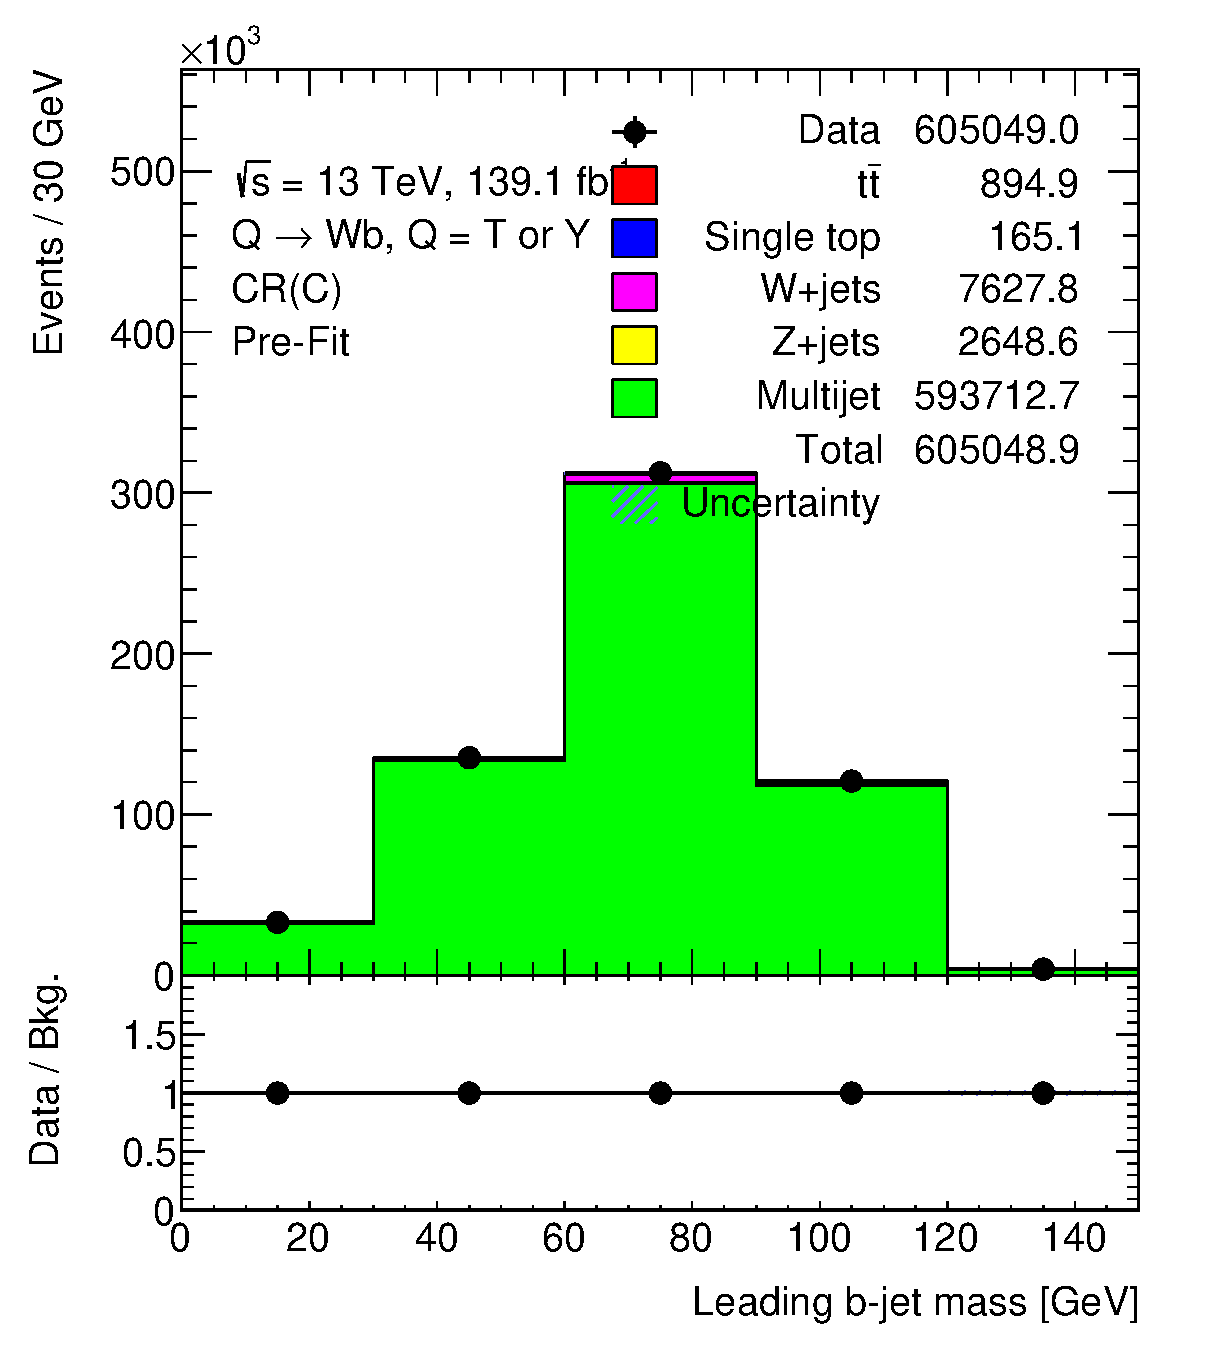
\includegraphics[width=\linewidth,height=\textheight,keepaspectratio]{CR_C_jet_m.eps}
		\caption{}
		\label{fig:app:cr_c:jet_m}
	\end{subfigure}
	\caption{A data/bkg.\ comparison of kinematic and reconstructed variables in CR C where the multijet background (in green) is calculated by Eqn.\ \ref{eqn:app} and the other backgrounds are from the MC simulation. The variables include (a) $p_{\text{T}}$ of $W$-tagged large-$R$ jet, (b) $p_{\text{T}}$ of leading $b$-tagged small-$R$ jet, (c) VLQ mass reconstructed from the kinematics of $W$-tagged large-$R$ jet and leading $b$-tagged small-$R$ jet, (d) $\eta$ distribution of $W$-tagged large-$R$ jet, (e) mass of $W$-tagged large-$R$ jet, and (f) mass of leading $b$-tagged small-$R$ jet.}
	\label{fig:app:cr_c}
\end{figure}








\begin{figure}[hbt!]
	\centering
	\graphicspath{{figs/appendix/CRD/}}
	\begin{subfigure}{.35\textwidth}
		\centering
		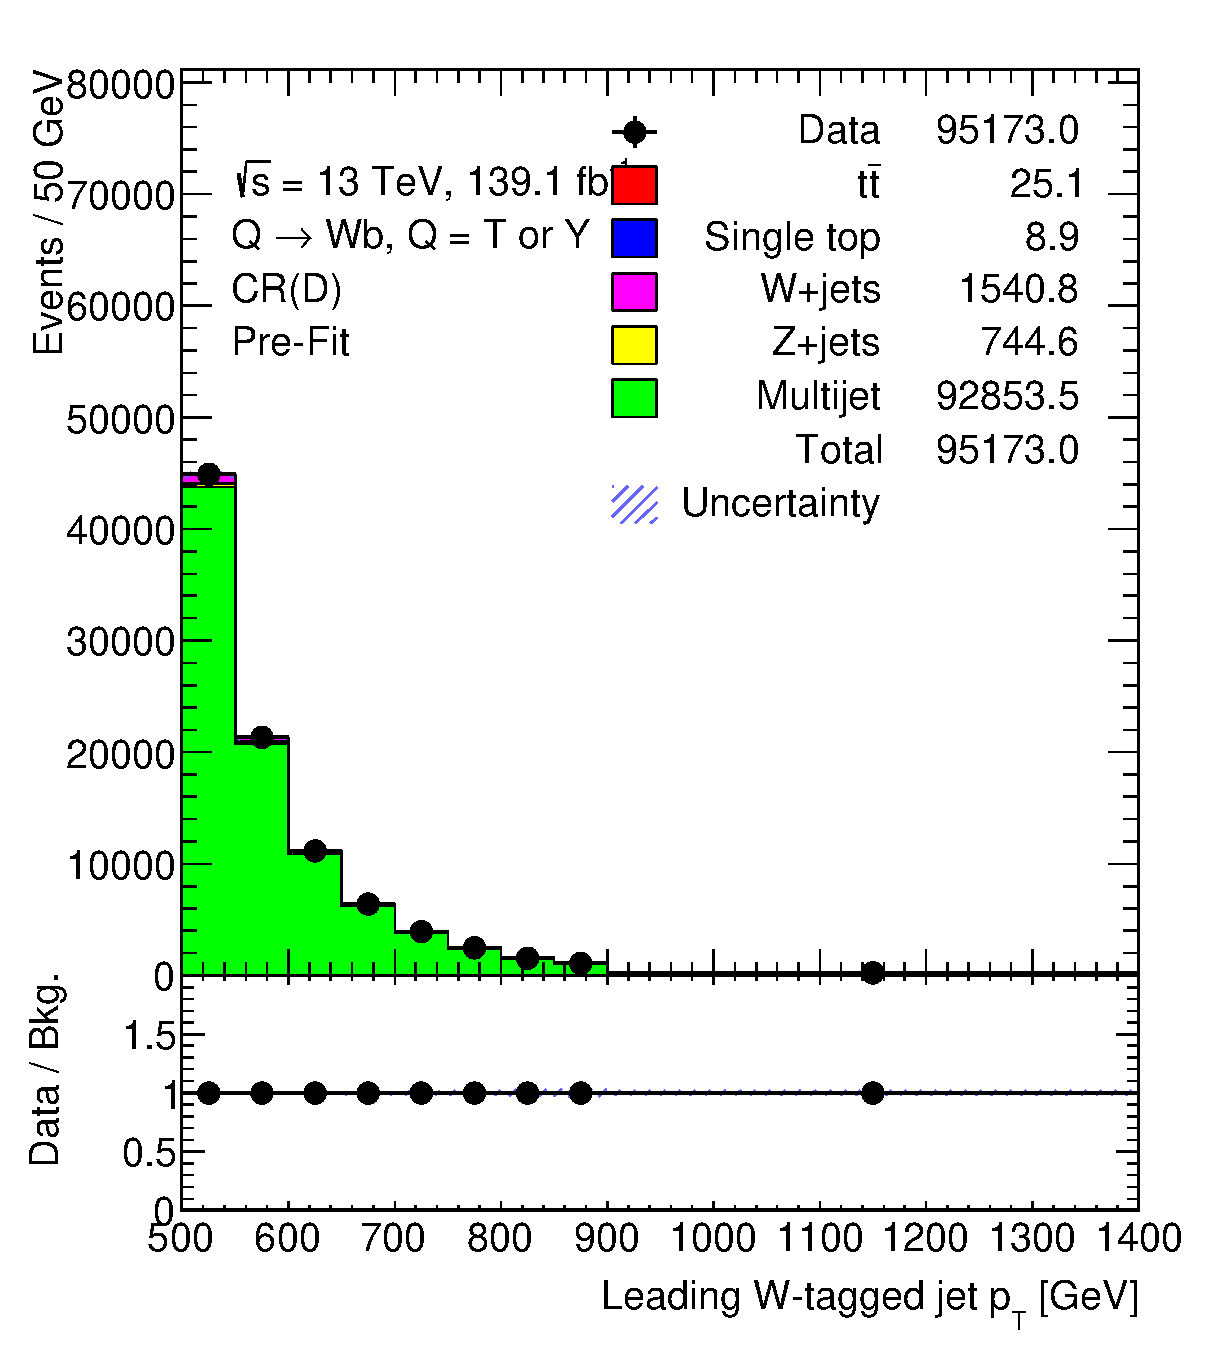
\includegraphics[width=\linewidth,height=\textheight,keepaspectratio]{CR_D_ljet_pt.eps}
		\caption{}
		\label{fig:app:cr_d:ljet_pt}
	\end{subfigure}\hspace{0.6cm}
	\begin{subfigure}{.35\textwidth}
		\centering
		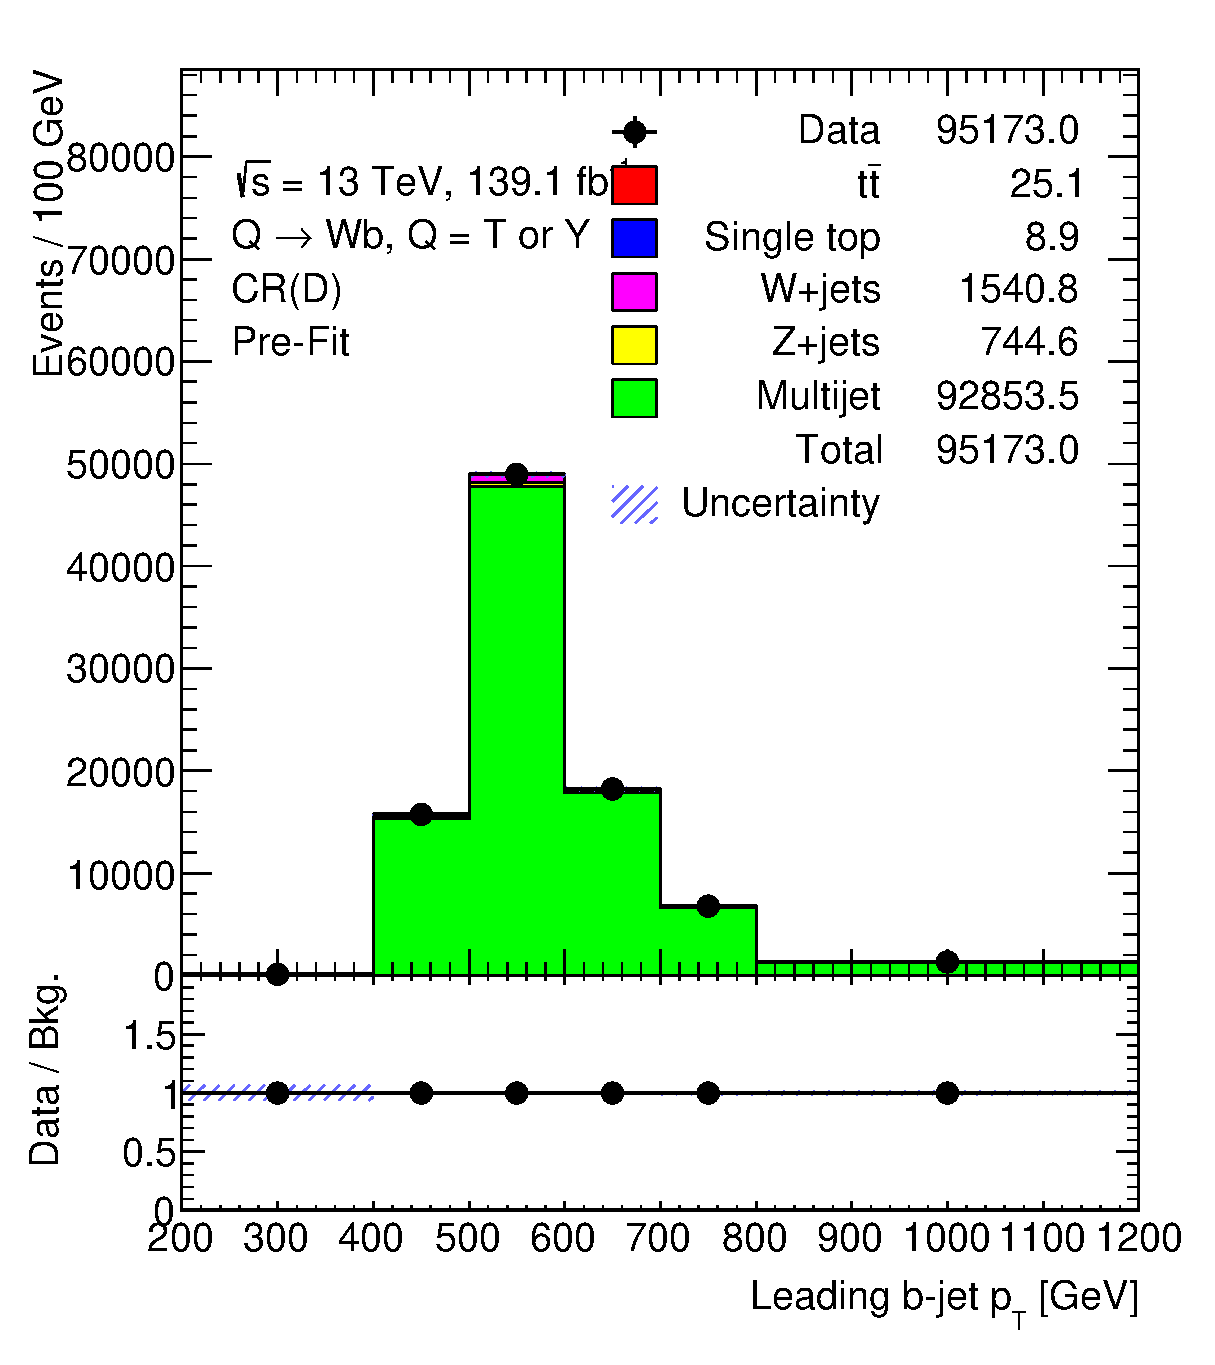
\includegraphics[width=\linewidth,height=\textheight,keepaspectratio]{CR_D_jet_pt.eps}
		\caption{}
		\label{fig:app:cr_d:jet_pt}
	\end{subfigure}
	\begin{subfigure}{.35\textwidth}
		\centering
		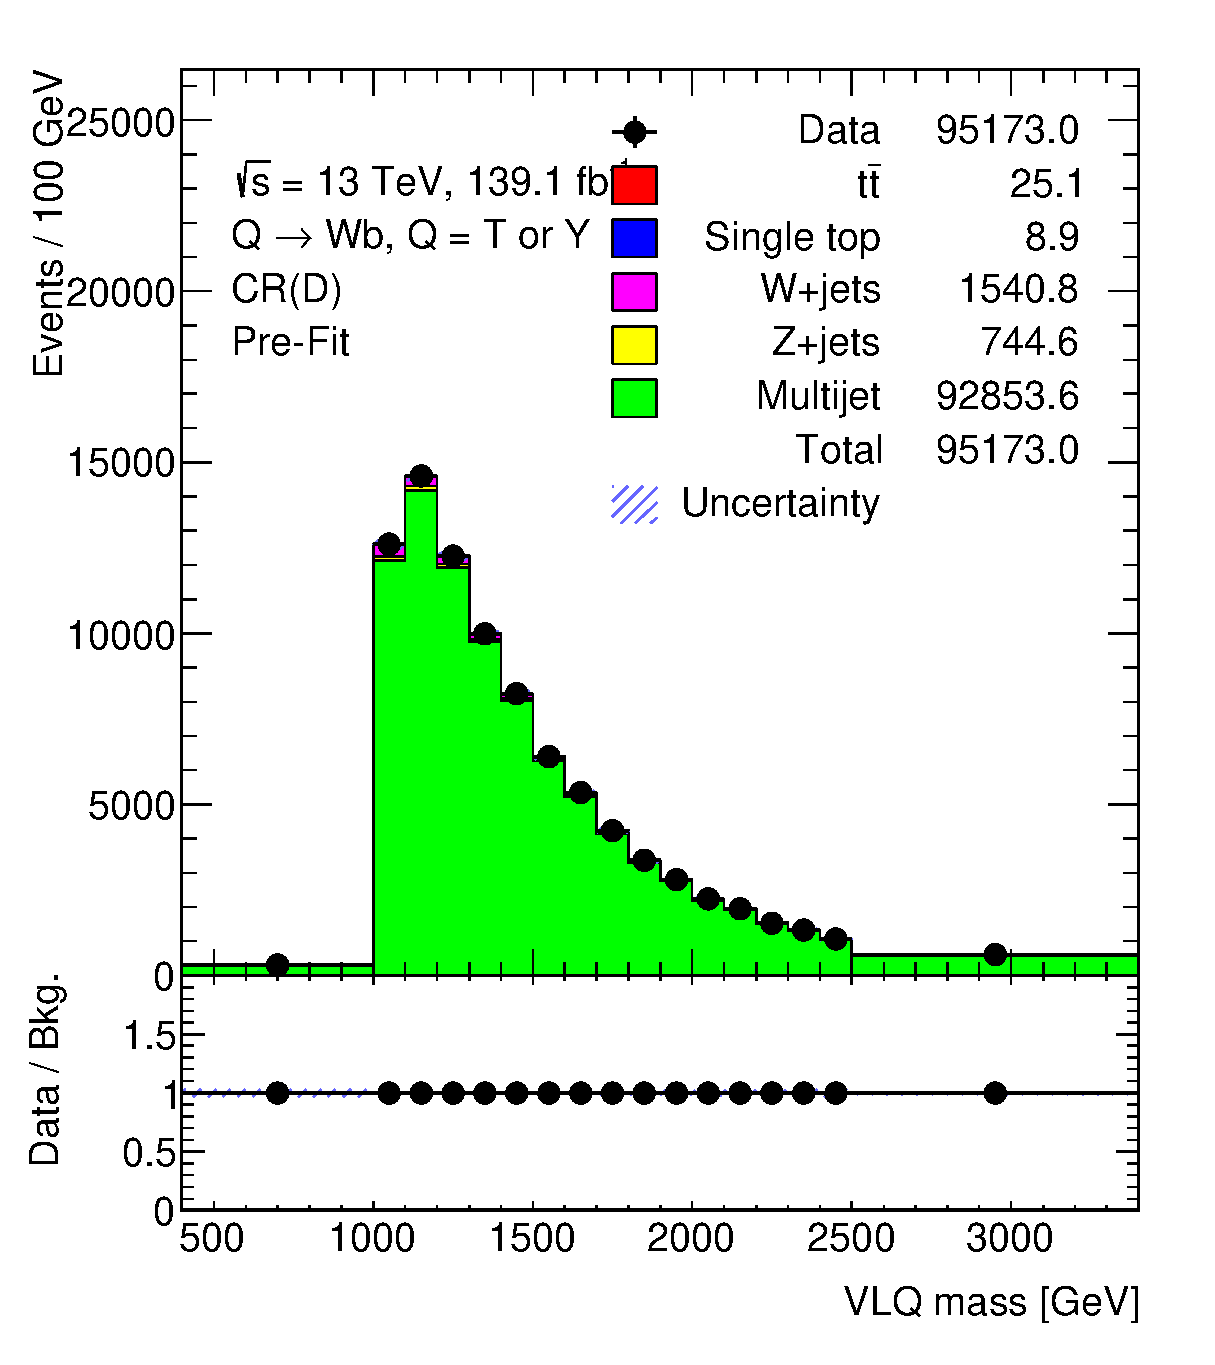
\includegraphics[width=\linewidth,height=\textheight,keepaspectratio]{CR_D_VLQM.eps}
		\caption{}
		\label{fig:app:cr_d:VLQM}
	\end{subfigure}\hspace{0.6cm}
	\begin{subfigure}{.35\textwidth}
		\centering
		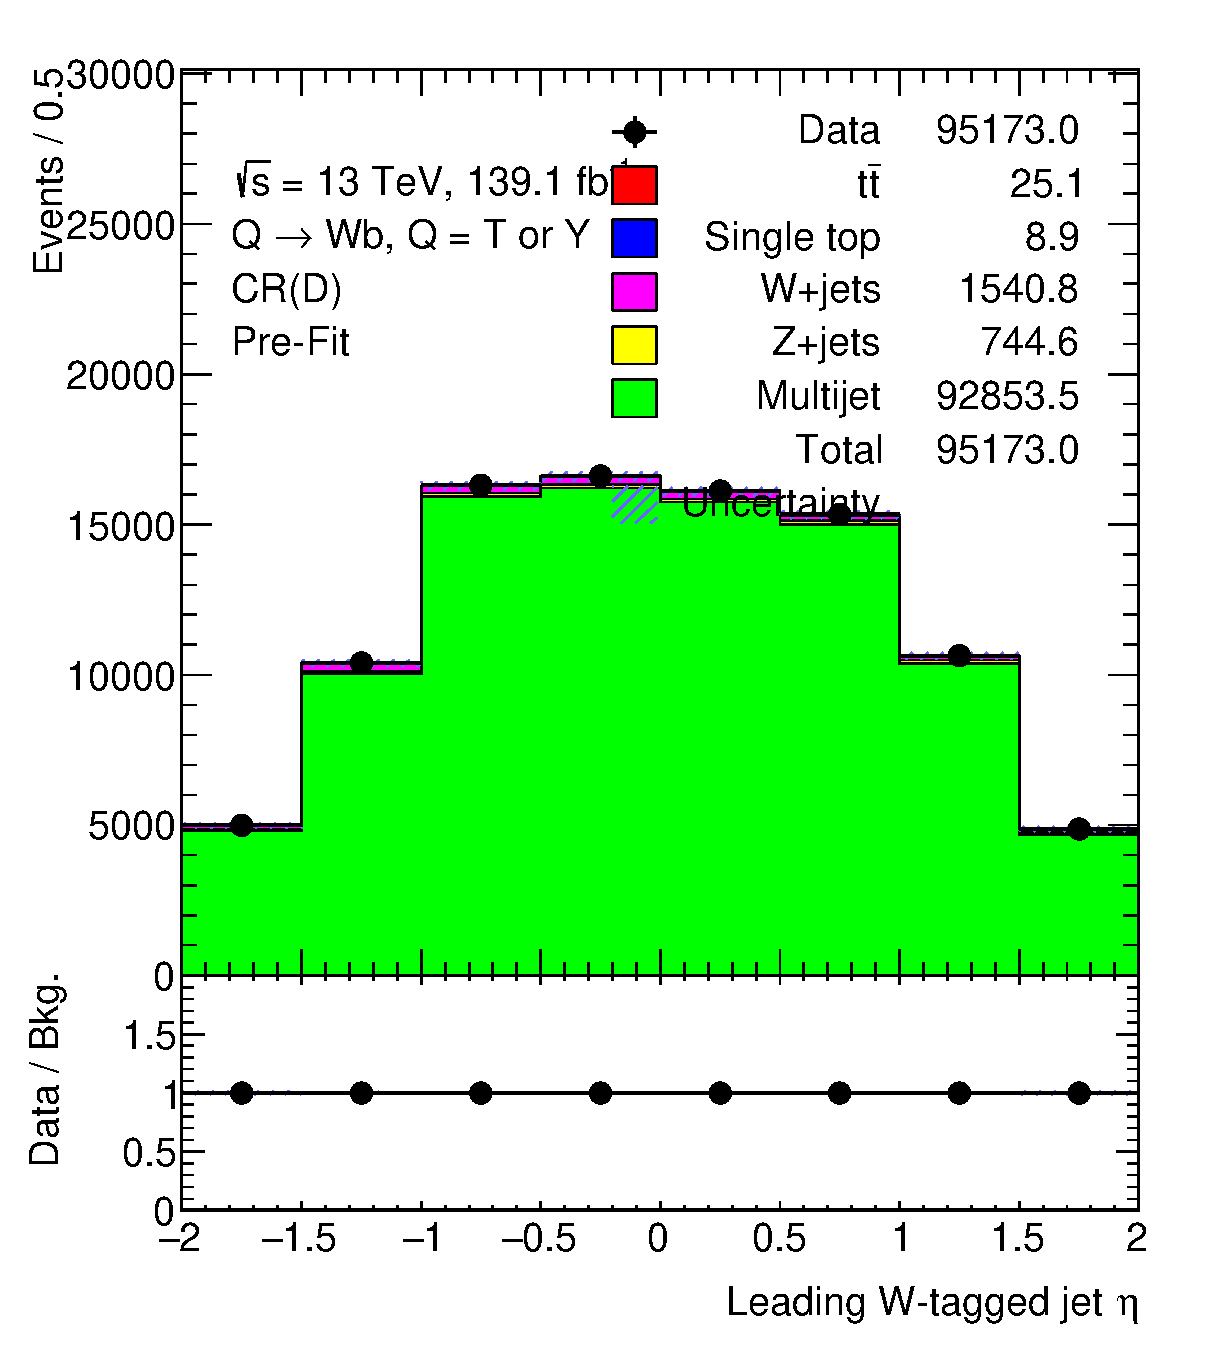
\includegraphics[width=\linewidth,height=\textheight,keepaspectratio]{CR_D_ljet_eta.eps}
		\caption{}
		\label{fig:app:cr_d:ljet_eta}
	\end{subfigure}
	\begin{subfigure}{.35\textwidth}
		\centering
		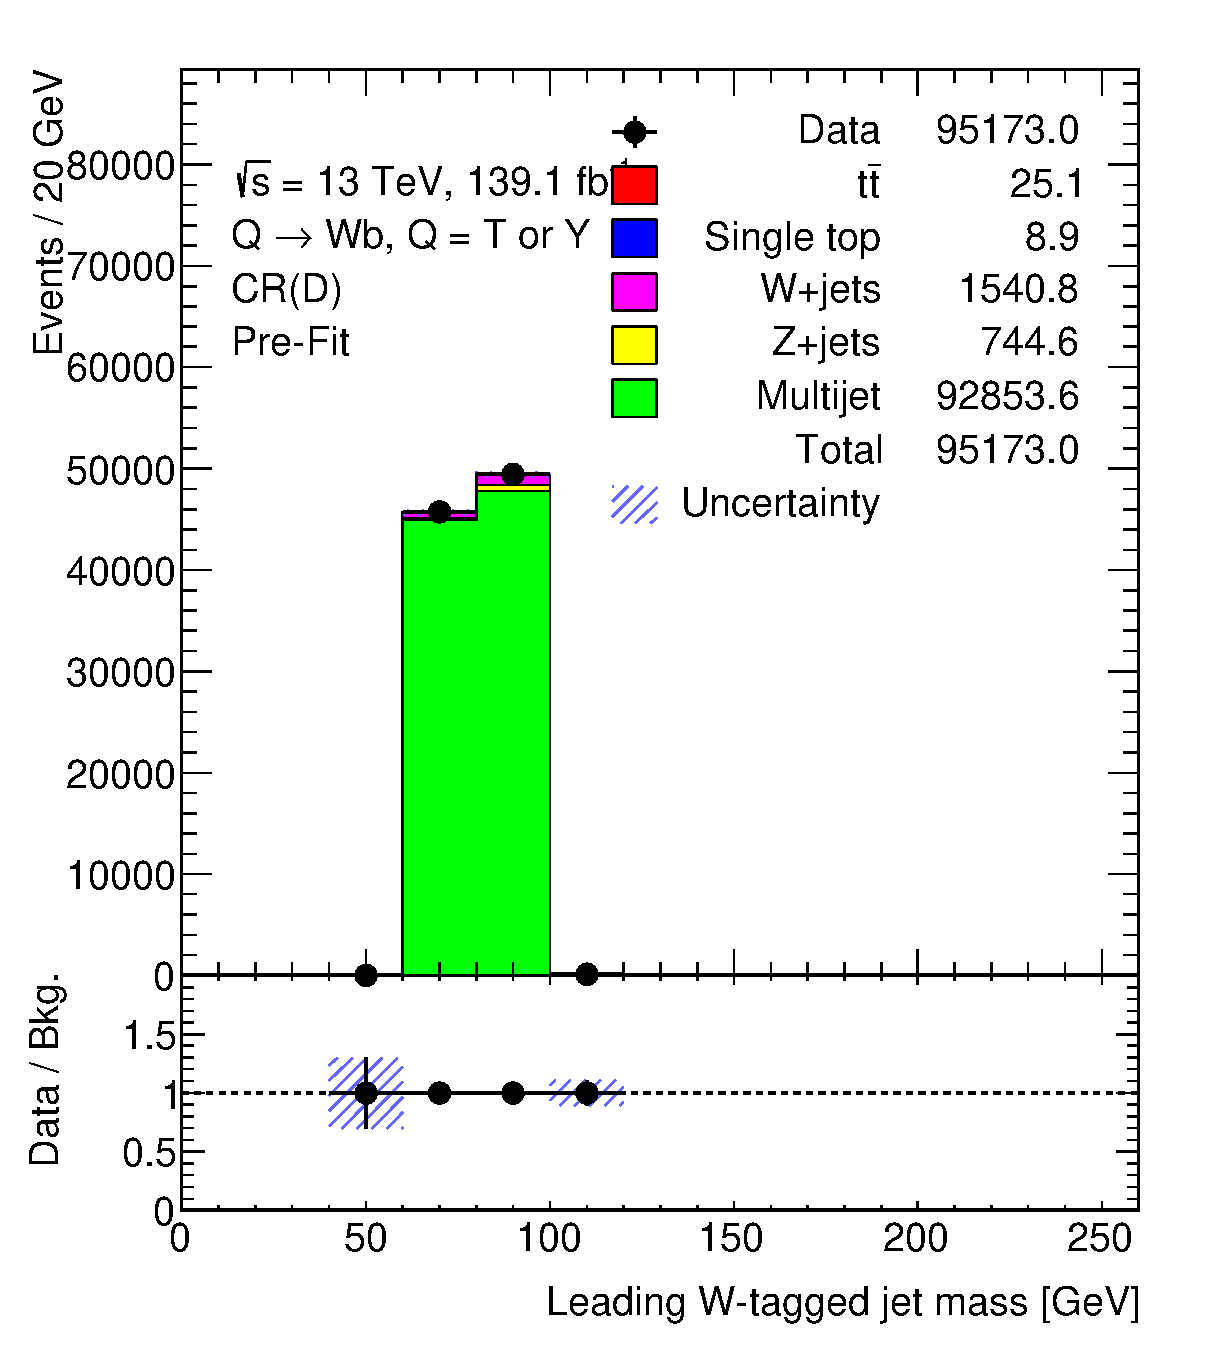
\includegraphics[width=\linewidth,height=\textheight,keepaspectratio]{CR_D_ljet_m.eps}
		\caption{}
		\label{fig:app:cr_d:ljet_m}
	\end{subfigure}\hspace{0.6cm}
	\begin{subfigure}{.35\textwidth}
		\centering
		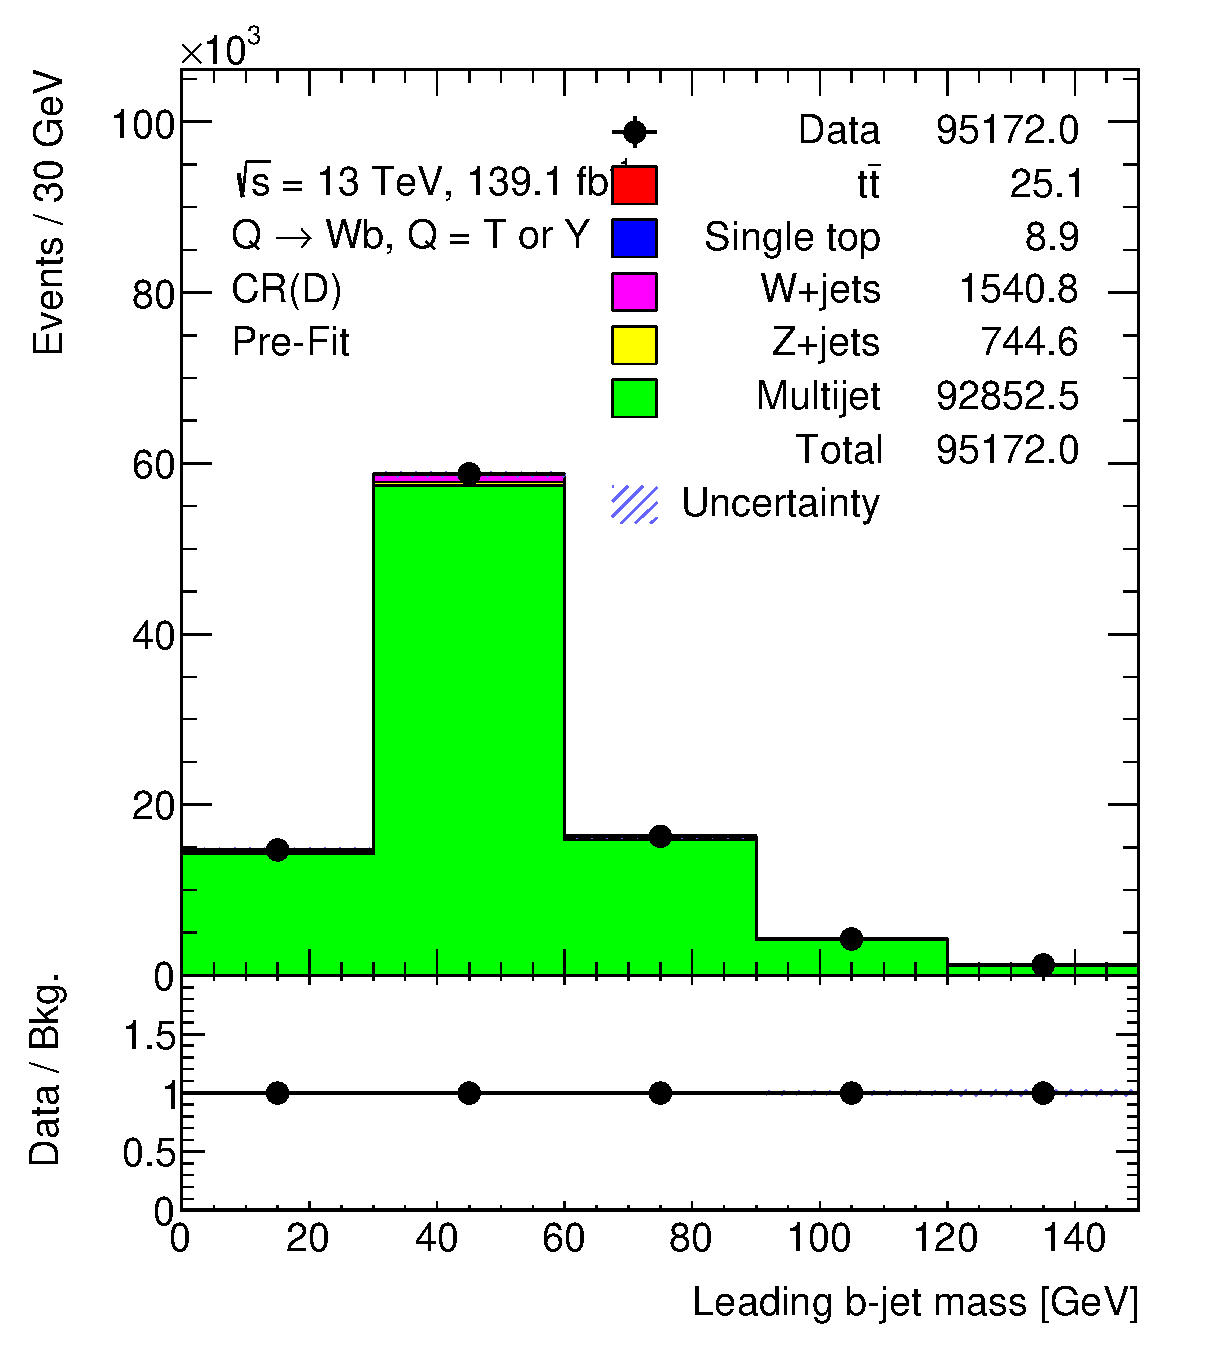
\includegraphics[width=\linewidth,height=\textheight,keepaspectratio]{CR_D_jet_m.eps}
		\caption{}
		\label{fig:app:cr_d:jet_m}
	\end{subfigure}
	\caption{A data/bkg.\ comparison of kinematic and reconstructed variables in CR D where the multijet background (in green) is calculated by Eqn.\ \ref{eqn:app} and the other backgrounds are from the MC simulation. The variables include (a) $p_{\text{T}}$ of $W$-tagged large-$R$ jet, (b) $p_{\text{T}}$ of leading $b$-tagged small-$R$ jet, (c) VLQ mass reconstructed from the kinematics of $W$-tagged large-$R$ jet and leading $b$-tagged small-$R$ jet, (d) $\eta$ distribution of $W$-tagged large-$R$ jet, (e) mass of $W$-tagged large-$R$ jet, and (f) mass of leading $b$-tagged small-$R$ jet.}
	\label{fig:app:cr_d}
\end{figure}





\begin{figure}[hbt!]
	\centering
	\graphicspath{{figs/appendix/CRD1/}}
	\begin{subfigure}{.35\textwidth}
		\centering
		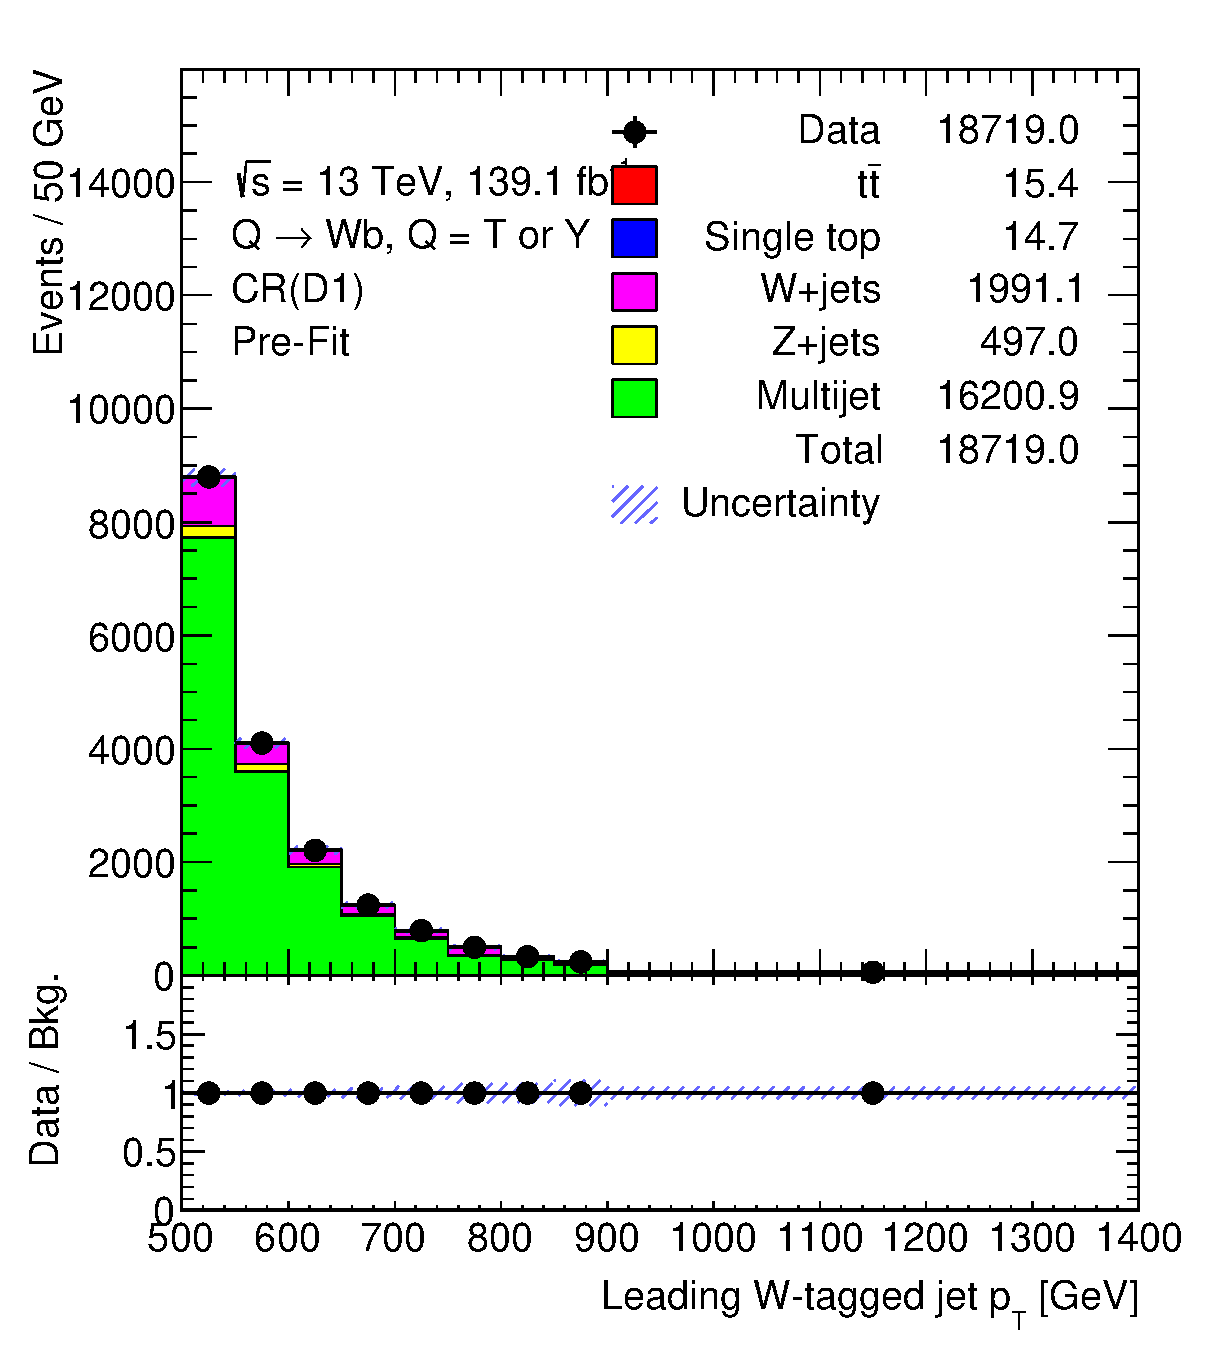
\includegraphics[width=\linewidth,height=\textheight,keepaspectratio]{CR_D1_ljet_pt.eps}
		\caption{}
		\label{fig:app:cr_d1:ljet_pt}
	\end{subfigure}\hspace{0.6cm}
	\begin{subfigure}{.35\textwidth}
		\centering
		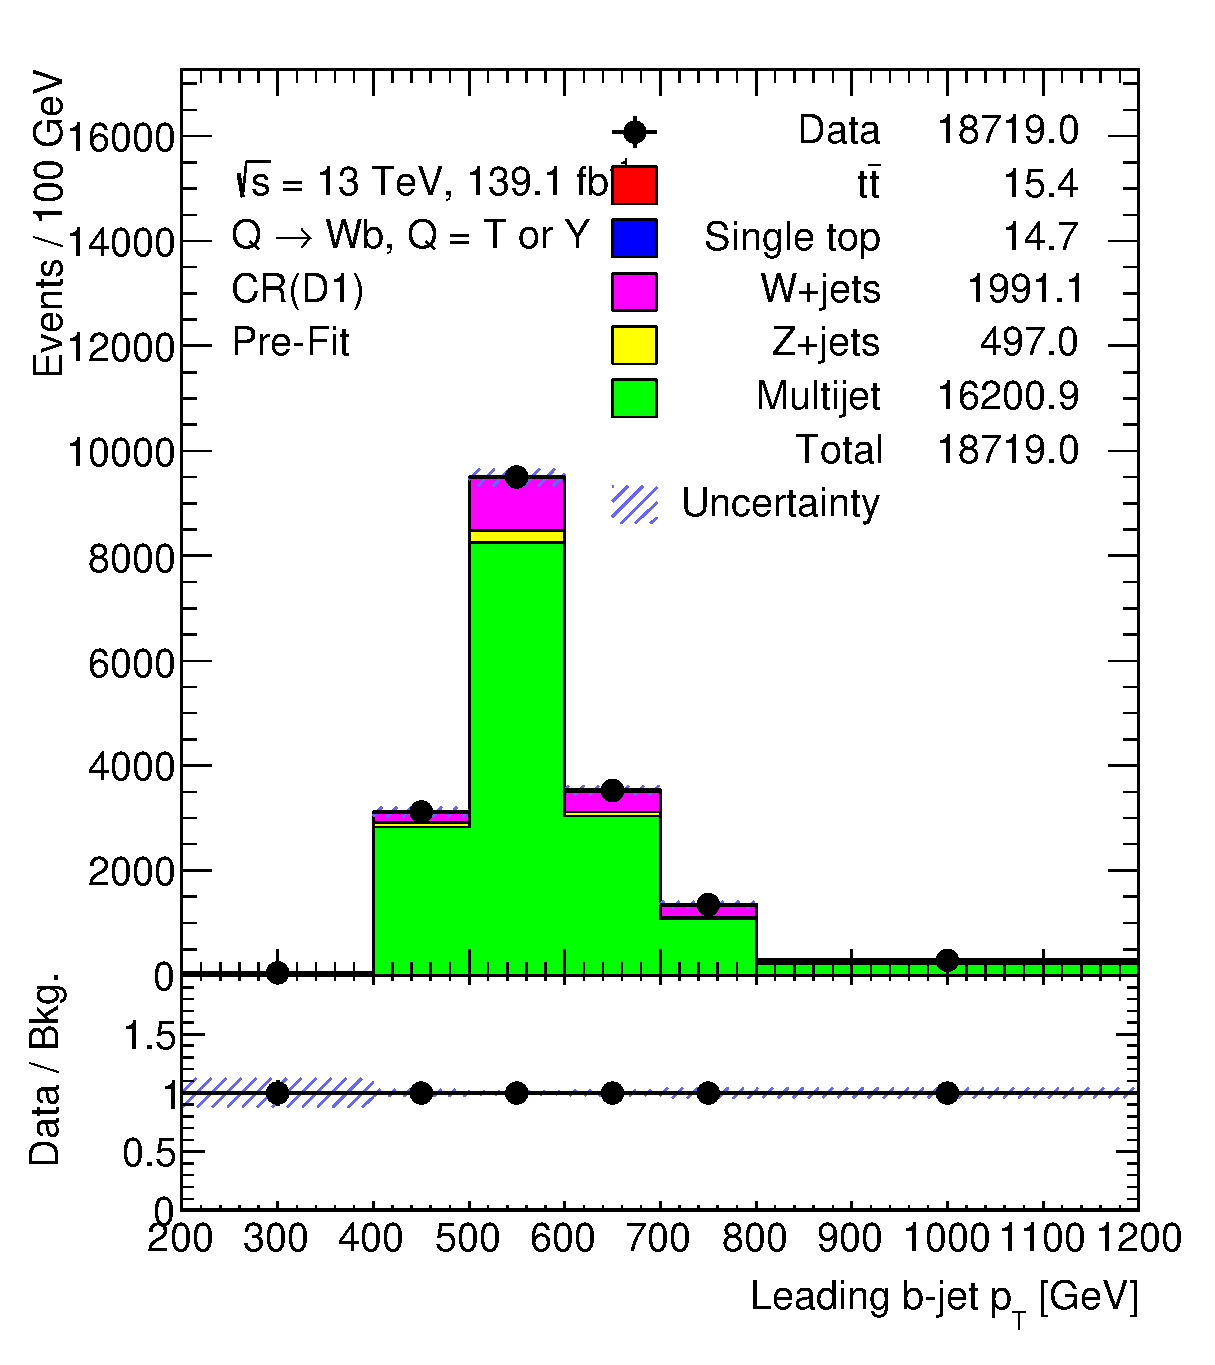
\includegraphics[width=\linewidth,height=\textheight,keepaspectratio]{CR_D1_jet_pt.eps}
		\caption{}
		\label{fig:app:cr_d1:jet_pt}
	\end{subfigure}
	\begin{subfigure}{.35\textwidth}
		\centering
		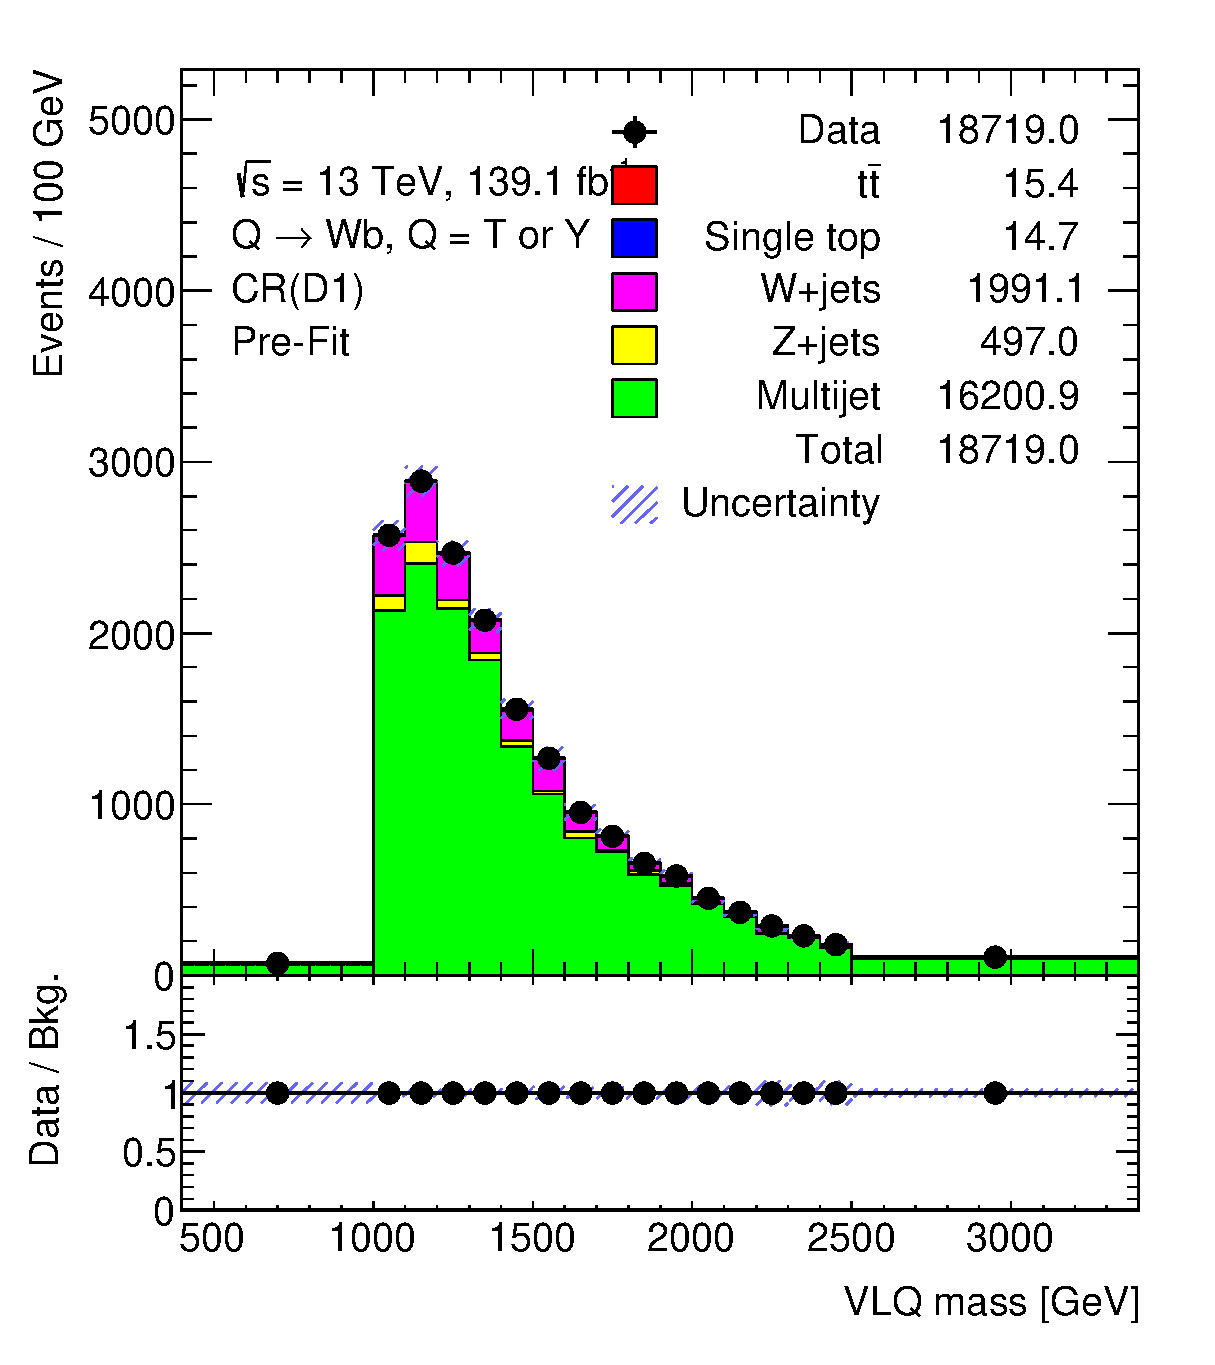
\includegraphics[width=\linewidth,height=\textheight,keepaspectratio]{CR_D1_VLQM.eps}
		\caption{}
		\label{fig:app:cr_d1:VLQM}
	\end{subfigure}\hspace{0.6cm}
	\begin{subfigure}{.35\textwidth}
		\centering
		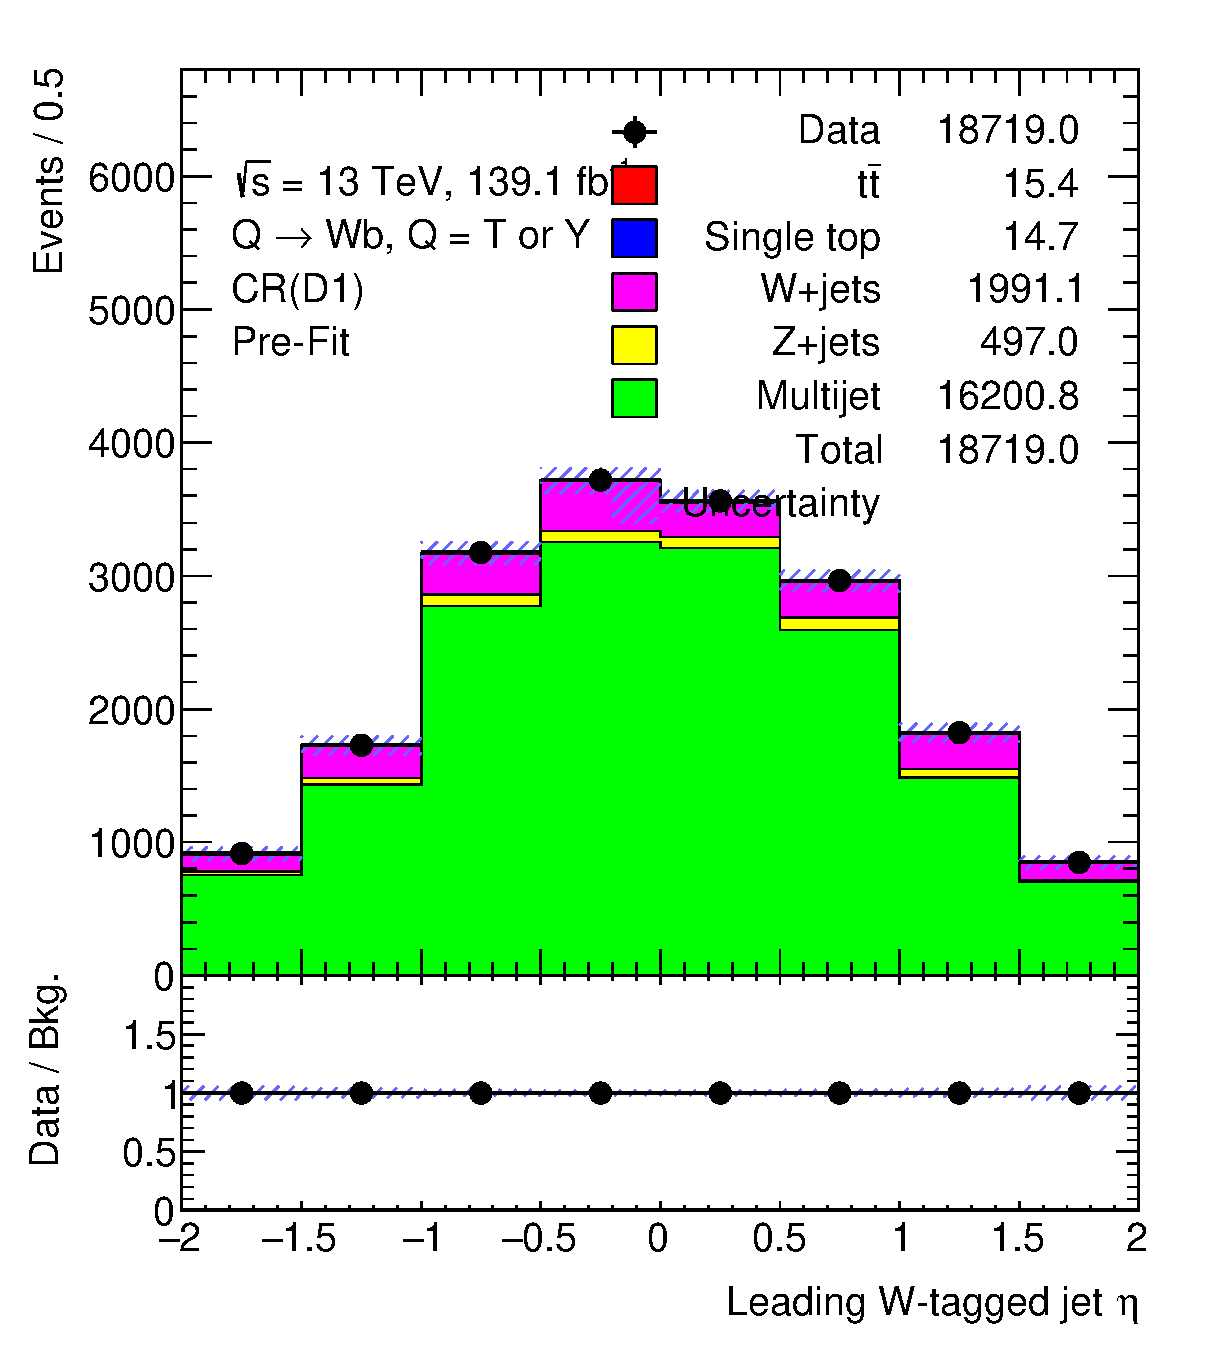
\includegraphics[width=\linewidth,height=\textheight,keepaspectratio]{CR_D1_ljet_eta.eps}
		\caption{}
		\label{fig:app:cr_d1:ljet_eta}
	\end{subfigure}
	\begin{subfigure}{.35\textwidth}
		\centering
		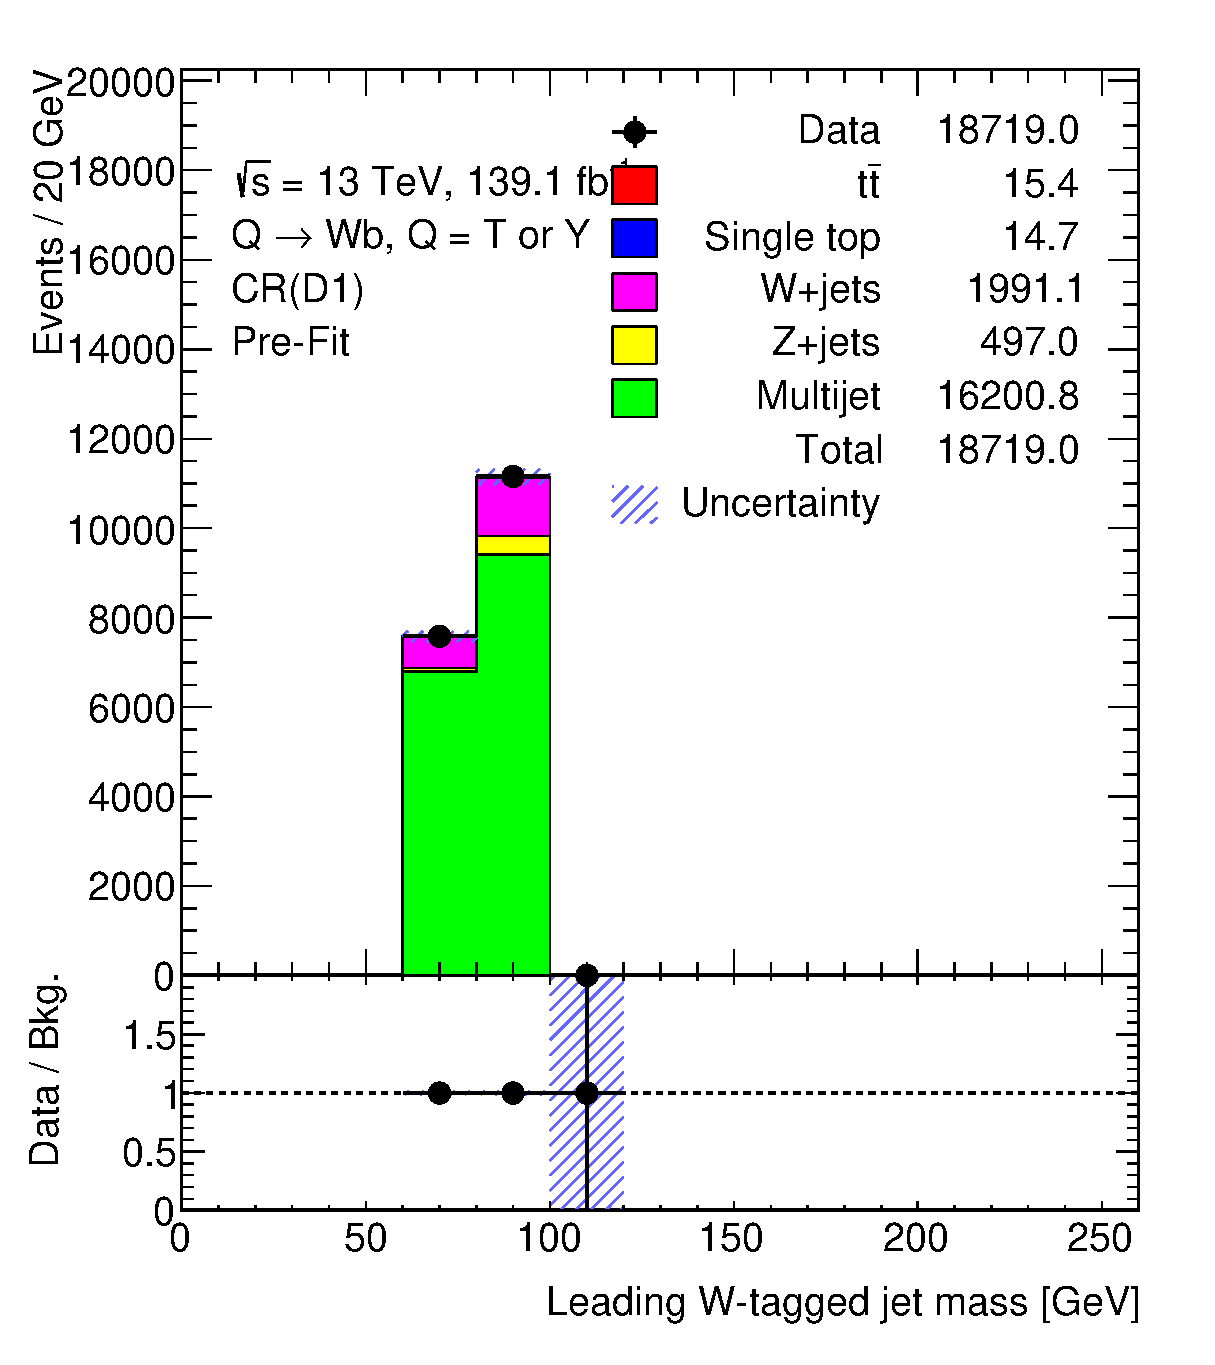
\includegraphics[width=\linewidth,height=\textheight,keepaspectratio]{CR_D1_ljet_m.eps}
		\caption{}
		\label{fig:app:cr_d1:ljet_m}
	\end{subfigure}\hspace{0.6cm}
	\begin{subfigure}{.35\textwidth}
		\centering
		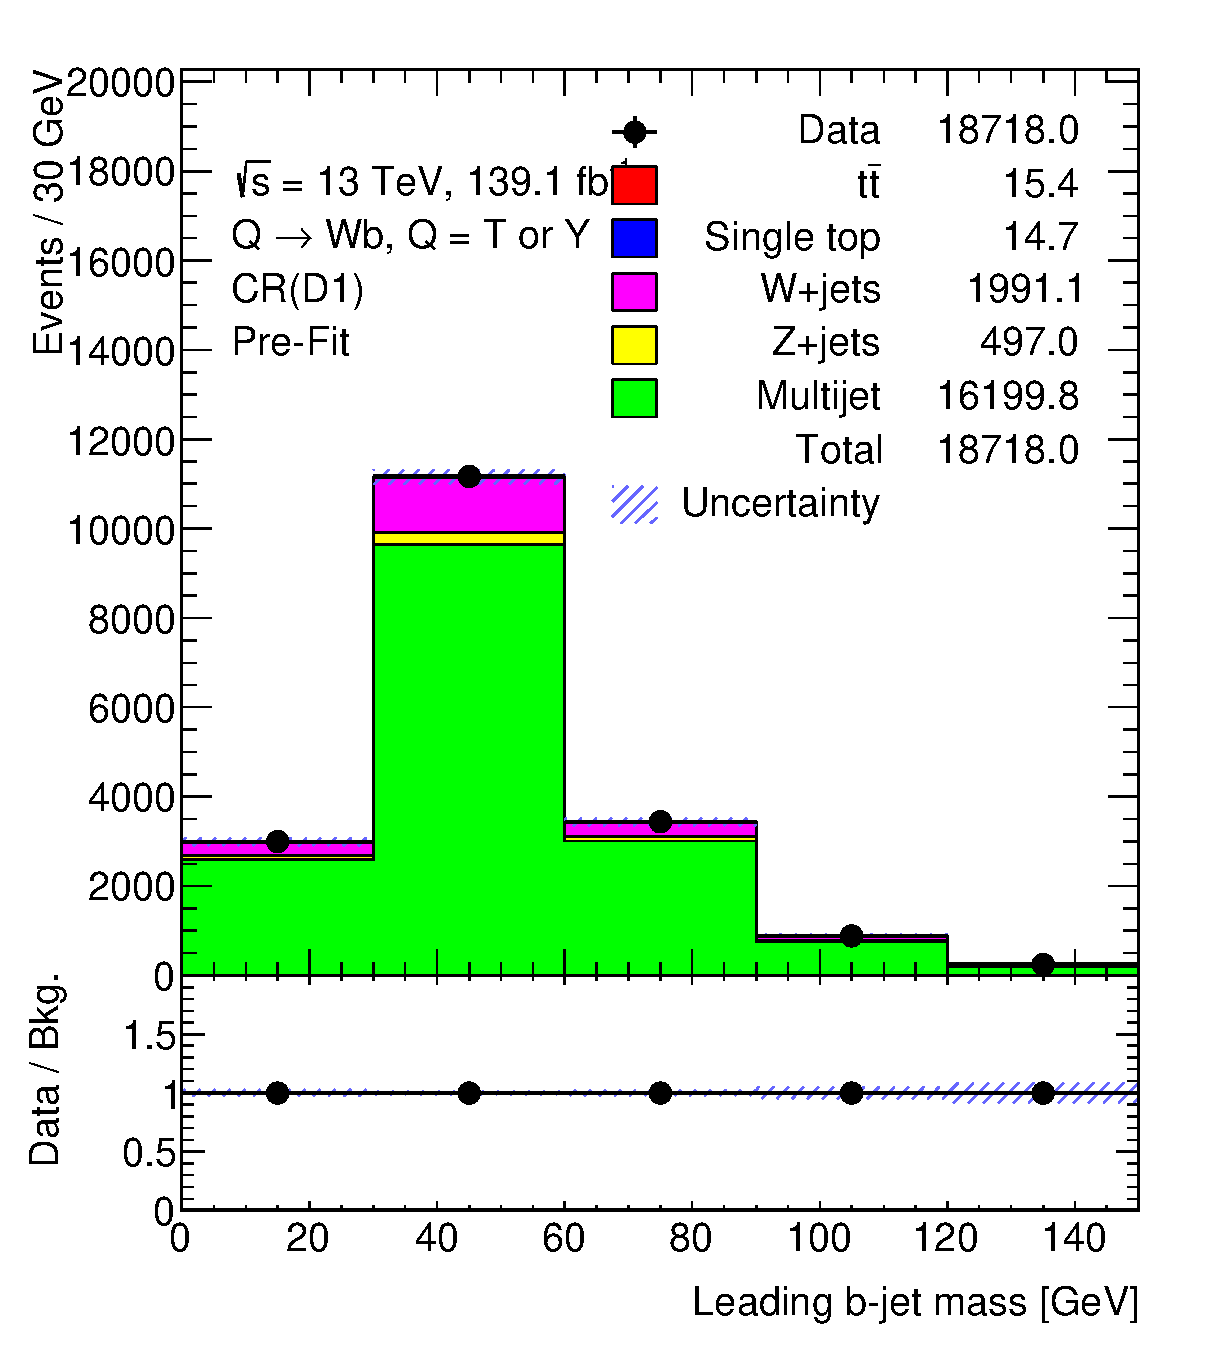
\includegraphics[width=\linewidth,height=\textheight,keepaspectratio]{CR_D1_jet_m.eps}
		\caption{}
		\label{fig:app:cr_d1:jet_m}
	\end{subfigure}
	\caption{A data/bkg.\ comparison of kinematic and reconstructed variables in CR D1 where the multijet background (in green) is calculated by Eqn.\ \ref{eqn:app} and the other backgrounds are from the MC simulation. The variables include (a) $p_{\text{T}}$ of $W$-tagged large-$R$ jet, (b) $p_{\text{T}}$ of leading $b$-tagged small-$R$ jet, (c) VLQ mass reconstructed from the kinematics of $W$-tagged large-$R$ jet and leading $b$-tagged small-$R$ jet, (d) $\eta$ distribution of $W$-tagged large-$R$ jet, (e) mass of $W$-tagged large-$R$ jet, and (f) mass of leading $b$-tagged small-$R$ jet.}
	\label{fig:app:cr_d1}
\end{figure}

%%% Local Variables: 
%%% mode: latex
%%% TeX-master: "../mythesis"
%%% End: 

% \printbibliography[heading=subbibliography]

%------------------------------------------------------------------------------
% Declare lists of figures and tables and acknowledgements as backmatter
% Chapter/section numbers are turned off
\backmatter

\listoffigures
\listoftables

%------------------------------------------------------------------------------
% Print the glossary and list of acronyms
% \printglossaries

%------------------------------------------------------------------------------
% You could instead add your acknowledgements here - don't forget to
% also add them to \includeonly above
% %------------------------------------------------------------------------------
\chapter{Acknowledgements}
\label{sec:acknowledgements}
%------------------------------------------------------------------------------
In 2017, I had the fortune to come to Germany and study physics. This would not have been possible without Bonn-Cologne Graduate School, so I would like to thank the admission committee for giving me an opportunity to pursue my master degree in physics.

I would like to thank Prof.\ Dr.\ Ian C.\ Brock for giving me an opportunity to write my thesis in his group. There is no doubt that without his guidance, wisdom and direction over the course of my degree, this thesis would not have been possible. I would also like to thank Prof.\ Dr.\ Florian Bernlochner, who agreed to be my second referee for this thesis.

Furthermore, I would like to thank Prof.\ Dr.\ Heiko Lacker, Dr.\ Janet Dietrich and Ferdinand Schenck from the Berlin VLQ group for helping me to understand the analysis better and also for their fruitful discussions on my results.

A big thanks to Anjishnu Bandyopadhyay for his support right from the beginning, when he introduced me VLQs till the last day of my submission. I truly appreciate all of his efforts for helping me with all my queries irrespective of the time on the clock as well as the priceless discussions on physics-related topics during DPG and at CERN. It has been a pleasure working with him. I would also like to thank Dr.\ Regina Moles Valls and Dr.\ Rui Zhang for their guidance and motivation when I initially joined this group as an intern. I would like to thank Dr.\ Oleh Kivernyk for his valuable suggestions on my results on the ABCD method.

Next, I would like to thank Federico G.\ D.\ Capriles for proofreading my first draft of this thesis and giving me some good memories of card game evenings. I would also like to thank Tanja Holm for the priceless discussions on jets and Christian Kirfel for the general discussions on machine learning related topics as well as teaching me some basic German culture. I would also like to thank Chris Boever for always motivating me and constantly reminding me that I am the next one after him. I am also grateful to him for proofreading some parts of my first draft of this thesis. I would like to thank Hanna We for all the interesting discussions we had on Indian and Korean cultures while sharing the same office. A special thanks to all the other members of the Brock group who were in the group during my days there, including but not limited to Nilima, Nicolas, Piet, Ellinor, Richard.

I would also like to thank everyone in the Desch group for the discussions during the Jamborees. A special thanks to all my friends and colleagues without them, my experience during my degree would not be as enjoyable.

Finally, I would like to thank my parents and family who are \SI{6000}{\kilo\meter} away from me but still their unconditional love and unlimited support encouraged me to start my venture; without them, it would not have been possible for me to manage and finish my studies.


%%% Local Variables: 
%%% mode: latex
%%% TeX-master: "../mythesis"
%%% End: 


%------------------------------------------------------------------------------
% CV needed when you submit your PhD thesis
% \definecolor{lightgray}{gray}{0.8}
\newcolumntype{L}{>{\raggedleft}p{0.15\textwidth}}
\newcolumntype{R}{p{0.8\textwidth}}
\newcommand\VRule{\color{lightgray}\vrule width 0.5pt}

\thispagestyle{empty}
\section*{Curriculum Vitae}

\subsection*{Personal Details}

\begin{tabular}{L!{\VRule}R}
Name & Johann Schmidt \\
Date of Birth &  \\
Email & abc@physik.uni-def.de \\
Family status & Single
\end{tabular}

\subsection*{Education}

\begin{tabular}{L!{\VRule}R}
1997--2003 & Abitur, ABC Secondary School, Hamburg, Germany\\
2004--2007 & BSc in Physics, Rheinische Friedrich-Wilhelms-Universität, Bonn, Germany.\\
2006 & CERN Summer Student, Geneva, Switzerland. \\
2007--2009 &  MSc in Physics Rheinische Friedrich-Wilhelms-Universität, Bonn, Germany. \\
2009--2012 &  PhD in Physics, Rheinische Friedrich-Wilhelms-Universität, Bonn, Germany. \\
2012 & Advanced Data Analysis School, Frankfurt, Germany.
\end{tabular}

\subsection*{Professional Experience}

\begin{tabular}{L!{\VRule}R}
2004 & Summer Student at CERN, Geneva, Switzerland. \\
2007--2012 & Doctoral work at the University of Bonn, Germany. \\
2008--2009 & Fieldwork at CERN, Geneva, Switzerland.\\
2011 & Talk at the Advanced Physics Conference, Timbucto
\end{tabular}

\subsection*{Languages}
\begin{tabular}{L!{\VRule}R}
German & Mother tongue \\
English & Fluent \\
Russian & Basic
\end{tabular}


\end{document}

%%% Local Variables:
%%% mode: latex
%%% TeX-master: t
%%% End:
